\documentclass[letter,8pt,landscape]{article}
\usepackage{fontspec}
\usepackage[T1]{fontenc}
\usepackage[frenchb]{babel} 
\usepackage{amssymb,amsmath,amsthm,amsfonts}
\usepackage{multicol,multirow}
\usepackage{calc}
\usepackage{graphicx}
\usepackage{ifthen}
\usepackage[landscape]{geometry}
\usepackage[colorlinks=true,citecolor=blue,linkcolor=blue]{hyperref}


\ifthenelse{\lengthtest { \paperwidth = 11in}}
    { \geometry{top=.1in,left=.1in,right=.1in,bottom=.1in} }
	{\ifthenelse{ \lengthtest{ \paperwidth = 297mm}}
		{\geometry{top=1cm,left=1cm,right=1cm,bottom=1cm} }
		{\geometry{top=1cm,left=1cm,right=1cm,bottom=1cm} }
	}
\pagestyle{empty}
\makeatletter
\renewcommand{\section}{\@startsection{section}{1}{0mm}%
                                {-1ex plus -.5ex minus -.2ex}%
                                {0.5ex plus .2ex}%x
                                {\normalfont\large\bfseries}}
\renewcommand{\subsection}{\@startsection{subsection}{2}{0mm}%
                                {-1explus -.5ex minus -.2ex}%
                                {0.5ex plus .2ex}%
                                {\normalfont\normalsize\bfseries}}
\renewcommand{\subsubsection}{\@startsection{subsubsection}{3}{0mm}%
                                {-1ex plus -.5ex minus -.2ex}%
                                {1ex plus .2ex}%
                                {\normalfont\small\bfseries}}
\makeatother
\setcounter{secnumdepth}{0}
\setlength{\parindent}{0pt}
\setlength{\parskip}{0pt plus 0.5ex}
% -----------------------------------------------------------------------

\begin{document}

\raggedright
\footnotesize

\begin{multicols}{3}
\setlength{\premulticols}{1pt}
\setlength{\postmulticols}{1pt}
\setlength{\multicolsep}{1pt}
\setlength{\columnsep}{2pt}

\vfill
\smallskip

  \section{General Concepts}
  Amdahl's law: $\text{overall speedup} = \frac{1}{(1-p) +
  \frac{p}{N}}$

  Gustafson's Law - Weak Scaling: $S = (1-p) + p \times N$

  Note that $N$: nproc and $p$: proportion of parallel code. Gustafson's Law
  addresses fixed problem size of Amdahl's law and instead gives the theoretical
  speedup a task gains from being parallelized. predacated that serial code in a
  parallelized environment remains fixed as problem scales as such assumes that
  problem scales with number of workers. Countering of serial component by
  increasing volume of computation. Amdahl's law is predicated under the strong
  scaling model where the problem size remains fixed.

  Little's Law: $L = p \times \lambda$
  
  Based on the idea of how to saturate compute volume. hid latency while
  performing other things during wait eg. memory access or pipeline stall.

  Computation Intensity q=$\frac{f}{m}$, f=$\textit{fp ops}$, m=$\textit{\# mem ops}$

  $\text{Memory instructions} = \text{memory}_\text{bw} \times \text{memory}_\text{latency}$

  $\text{Arithmetic Instructions} = \text{arith}_\text{throughput} \times \text{arith}_\text{latency}$

  $\text{Concurrency} = \text{memory}_\text{bandwidth} \times \text{memory}_\text{latency}$

  \subsection{Speedup \& Efficiency}


  GPU speedup: $S_\text{GPU} = \frac{\text{fastest CPU completion
  time}}{\text{completion time on GPU}}$

  Parallel Compute speedup: $S_p = \frac{\text{single threaded
  completion}}{\text{parallel completion}}$

  Efficiency: $E_p = \frac{S_p}{p}$ where $p$: nproc


  Scaled Speedup: $PT_p = T_1 + T_o$, where $T_1$ is serial runtime and $T_o$ is
  parallel overhead.

  Isoefficiency: There is some function $f(P) = N$ that specifies the problem
  size ($N$) that keeps parallel efficiency constant. given that efficiency is
  given as $E = \frac{S}{P} = \frac{1}{1 + \frac{T_o}{T_1}} = \frac{1}{1 +
  \frac{T_o}{Wt_c}} $ with $T_1 = Wt_c$ where $W$: problem size in operations
  and $t_c$: time per op. we note that $T_o$ is a function of $P$ as such $W$
  should grow as a function of $P$ as well. eg. with Fat tree topology $T_o =
  O(\log(P))$ -- network diameter

  \subsubsection{Performance Prediction}
  Computation time: $T_\text{comp} = D(n) + \frac{W(n) - D(n)}{p}$, where $W(n)$
  is the number of work nodes and $D(n)$ is nodes on critical path. Ratio
  implies how parallelizability it is $\frac{W(n)}{D(n)}$. eg, Matrix multiply
  -- $W(n) = n$: number of multiplies -- $D(n) = \log(n)$: reduction add. Ratio
  shows massive potential for parallelization

  Compute time: $T(1, (m,n)) =$ time for best serial algorithm on a $m\times n$
  problem. $T(p, (m,n)) = T(1,(m,n)) + T_\text{comm}$: runtime on $p$ processes
  where $(m,n) = \frac{N}{(p,q)}$ with $p\times q$ being process grid on
  $N\times N$ problem.
  $T_\gamma(p, (m,n)) = \frac{T(P,(m,n))}{m\cdot n\cdot \text{N iterations}}$.
  
  Grind time: parallel performance ignoring communication time
  $T_\text{comm}$



  \subsubsection{Super Linear Speedup}
  when $S_p > P \implies \frac{S_p}{p} = E_p > 1$. Real super linear scaling
  exiss when $P$ scales things such as memory/cache sizes/bandwidth or yields
  more network bandwidth. Can be faked with poor algorithm or measurement
  technique. often suggests a better serial algorithm exists since $S_p =
  \frac{T_s}{T_p}; E_p = \frac{S_p}{p} > 1 \implies T_s > p\times T_p$ meaning
  $T_s$ is not optimal and there exists some serial that could perform the
  parallel component and take less time than original.


  \subsection{Roofline Model}
  Peak performance for each processor is intrinsic based on clock speed with
  bandwidth determining how steep the slop is. $q = \frac{\text{Flops}}{\text{Bytes}}$.
  Where "bytes" is amount of memory operations and flops being the computation
  amount.
  \begin{center}
    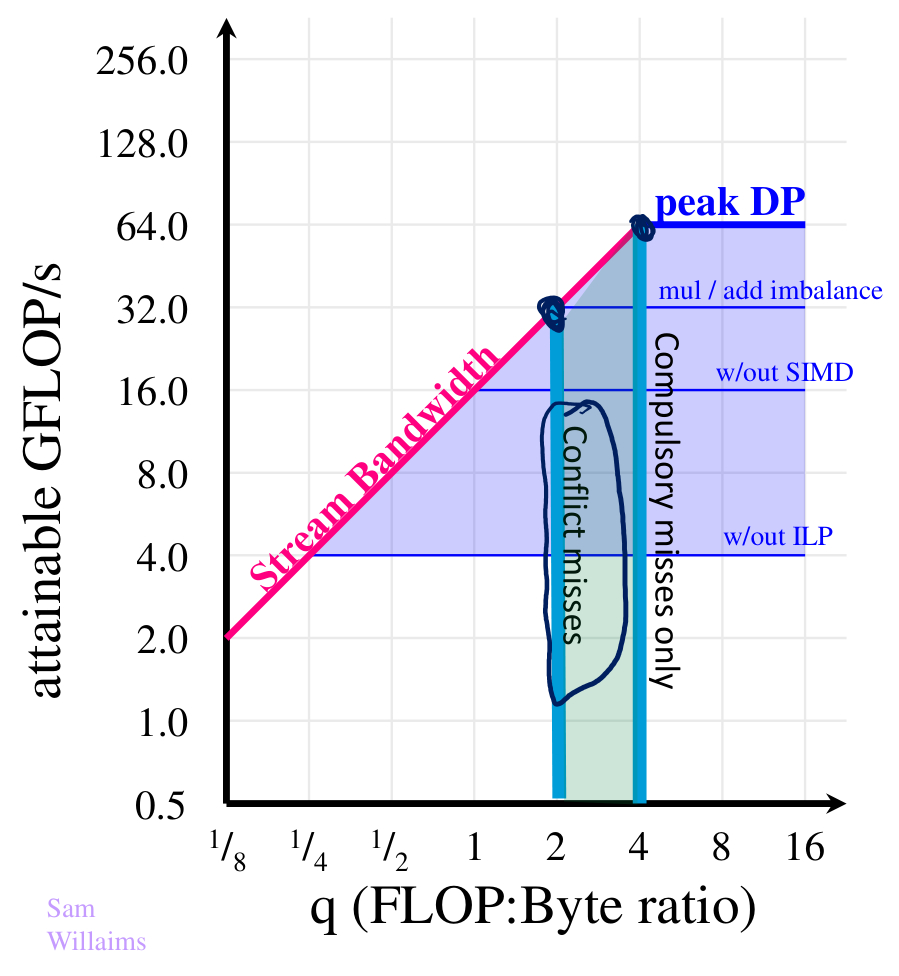
\includegraphics[width=1.5in]{images/roofline-eg.jpg}
  \end{center}
  

  \subsection{Memory Hierarchy}

  Layers of cache hierarchy are to tradeoff access speed and capacity.

  \begin{center}
    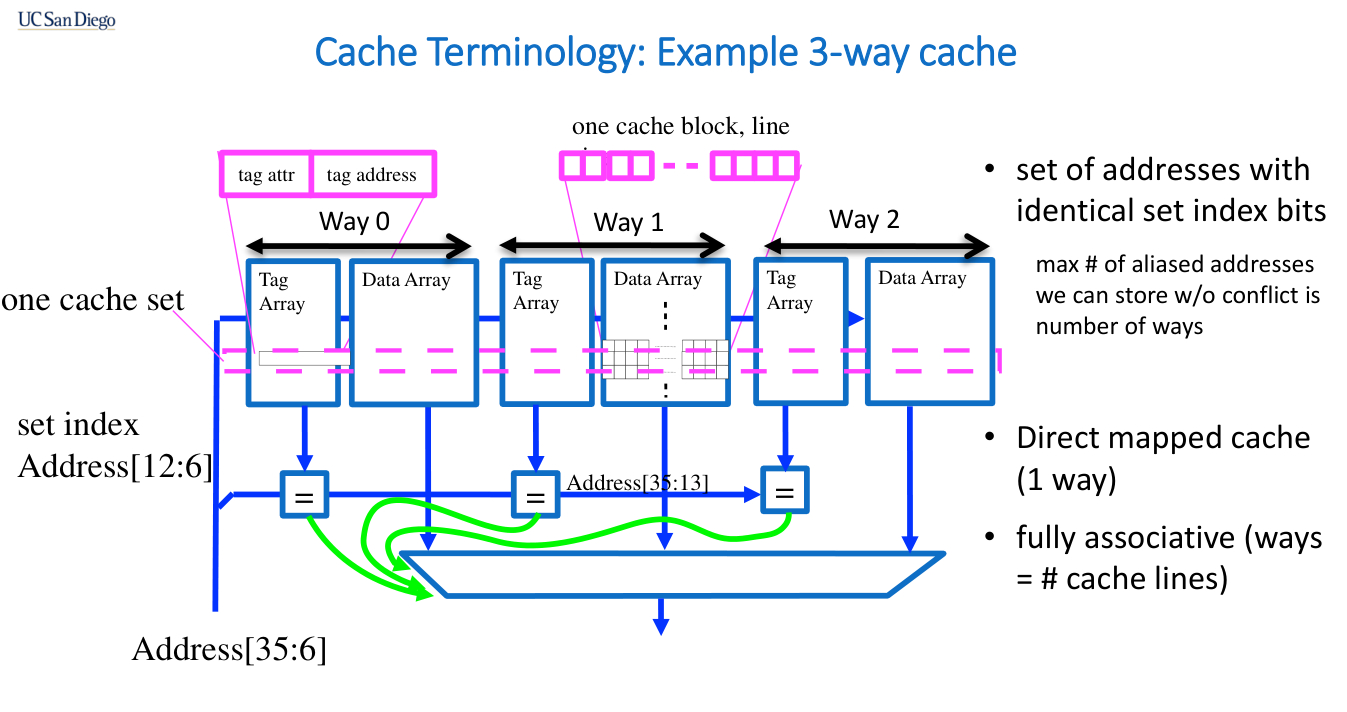
\includegraphics[width=\linewidth]{images/nway-cache.jpg}
  \end{center}
  3-way cache extends to $n$-way cache

  Cold miss: miss due to first access of data

  Capacity miss: miss due to cache being full

  Conflict miss: miss due to too many set aliases for memory addresses mapping
  to caches

  Temporal Cache locality: recent use of memory address

  Spatial Cache locality: use of a memory address is close to a previously used
  one

  One example of increasing spatial locality is packing, which can reduce caches misses:
  \begin{center}
    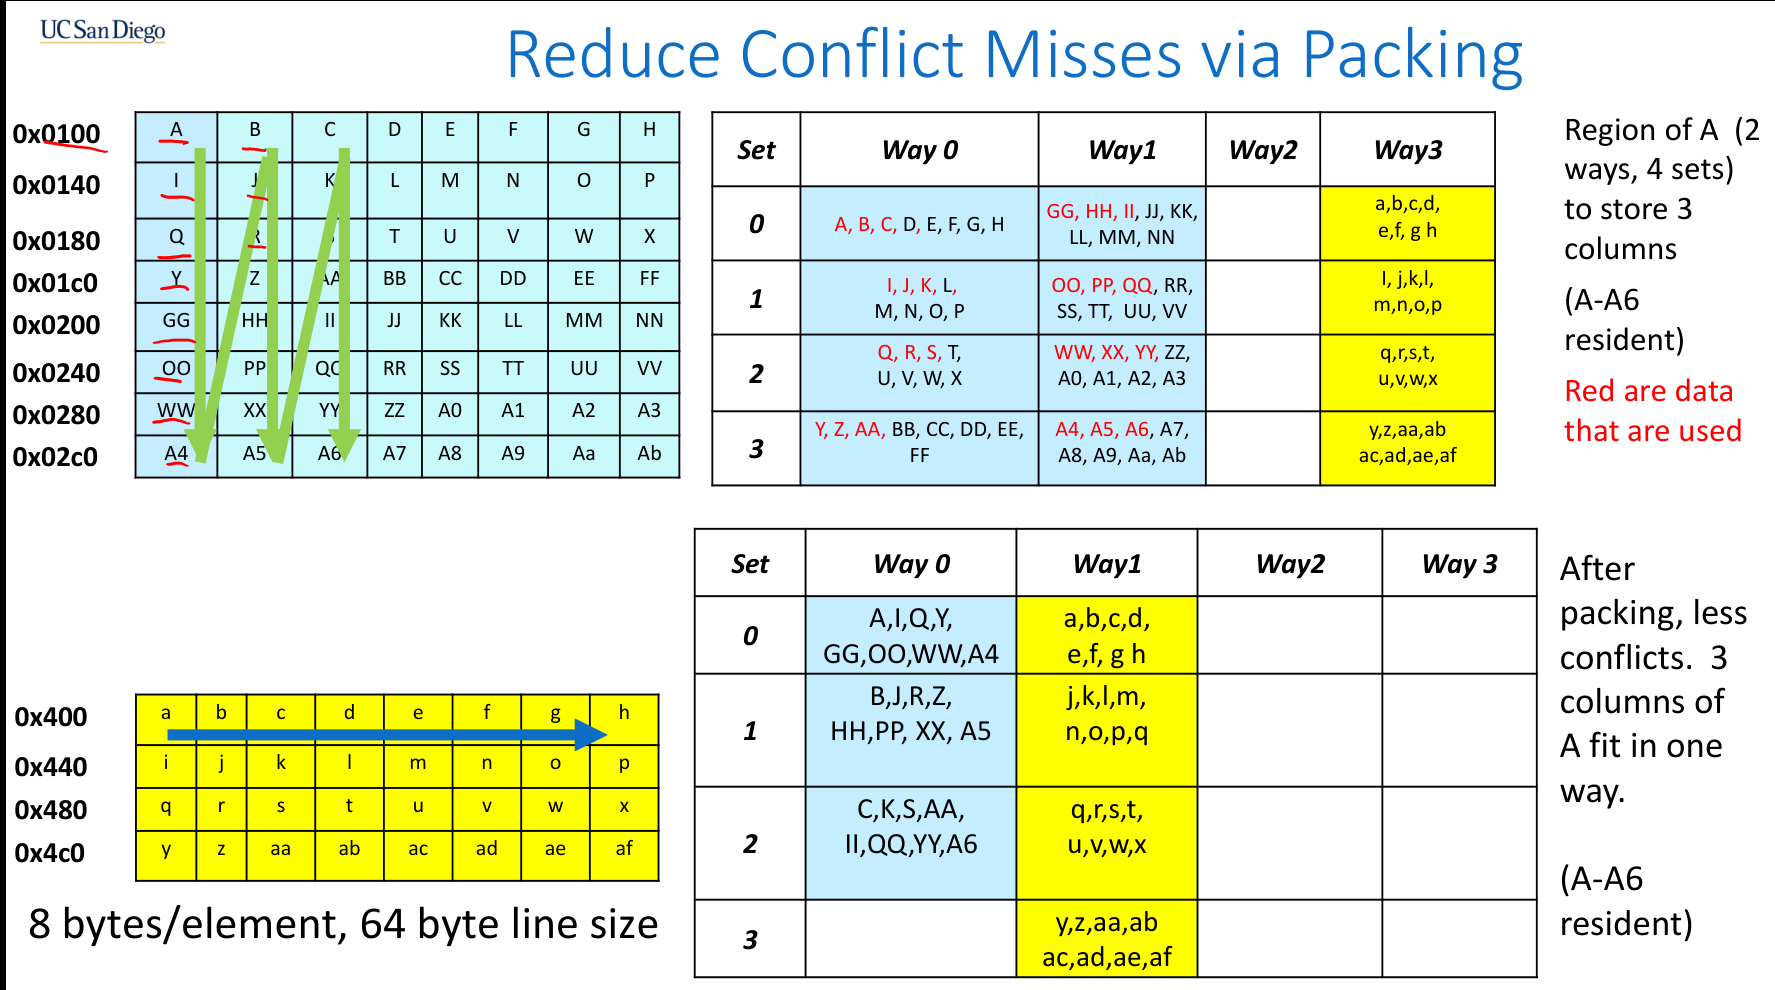
\includegraphics[width=2in]{images/packing.png}
  \end{center}

  \section{Matrix Multiply}
  Naive Matrix Mult: $q = \frac{2n^3}{n^3 + 3n^2}$. With $2n^3$: $n^3$ being
  iterating over elements of $A,B$ and $2$ from add and mult. $n^3$ comes from
  loading blocks of $B$ (hot loop), $n^2$ comes from loading blocks of $A$ and
  load and store to blocks of $C$.

  Blocking Matrix Mult: Same comp intensity as the naive just access pattern is
  more cache friendly. So performance ends up being some scalar fraction of
  Naive as $N$ increases.

  GOTOblas:
  \begin{center}
    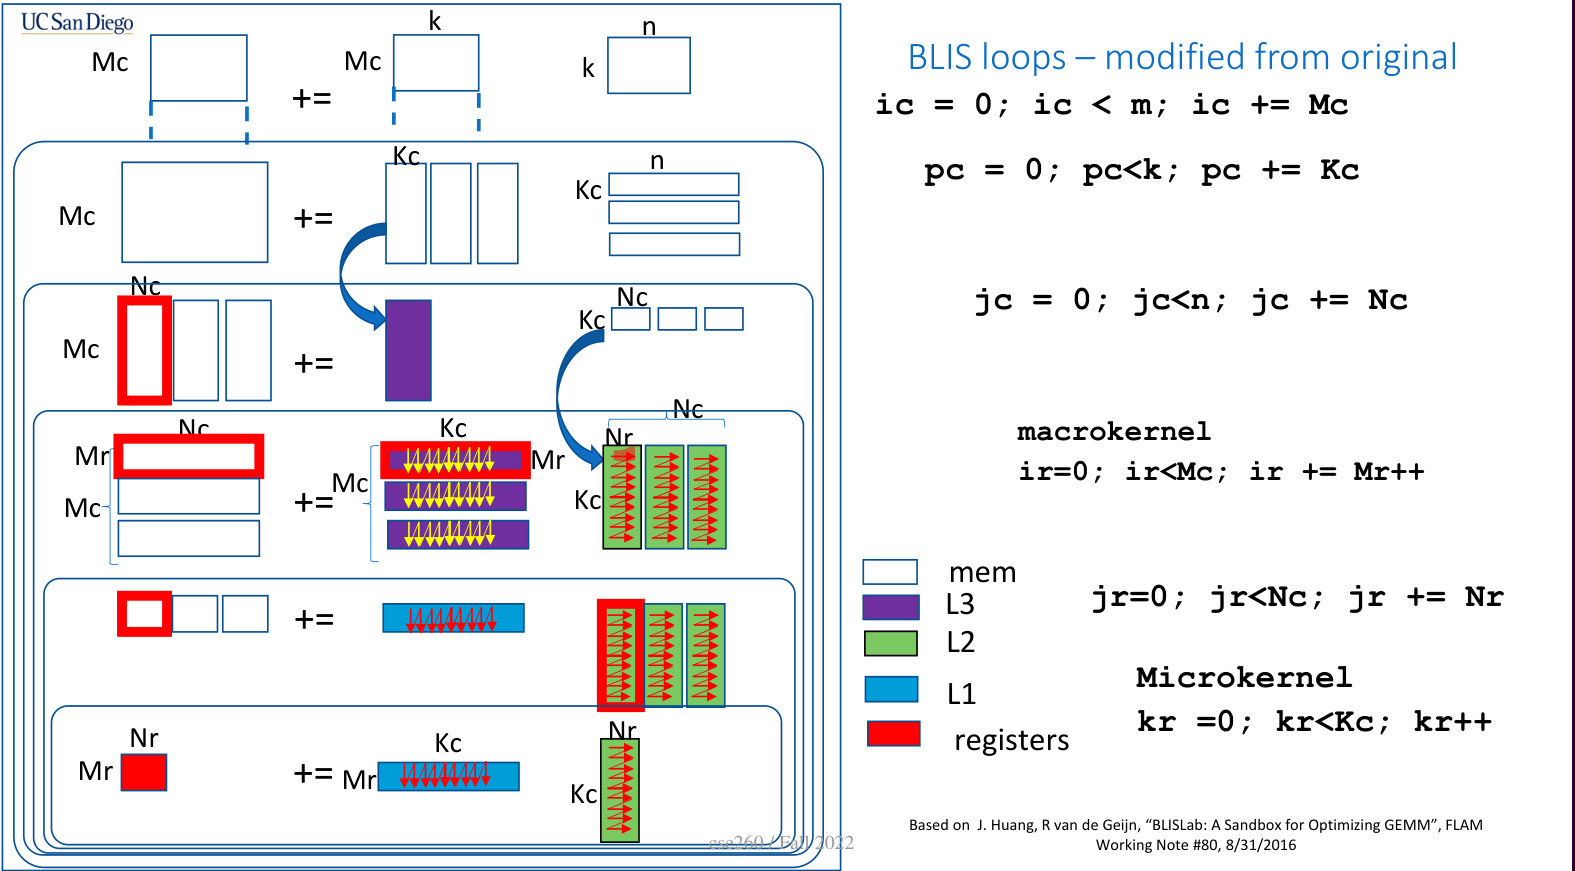
\includegraphics[width=2in]{images/gotoblas.jpg}
  \end{center}

  $q = \frac{2n^3}{(2N + 2) * \frac{n^2}{L}}$. Where $N$ is size of cached
  sub-matrix and $L$ is size of cache line. - $2N$ are operations neede for
  repacking. $+2$ is for an load and store of element of $C$

  \subsection{Parallel Matrix Multiply}

  \begin{center}
    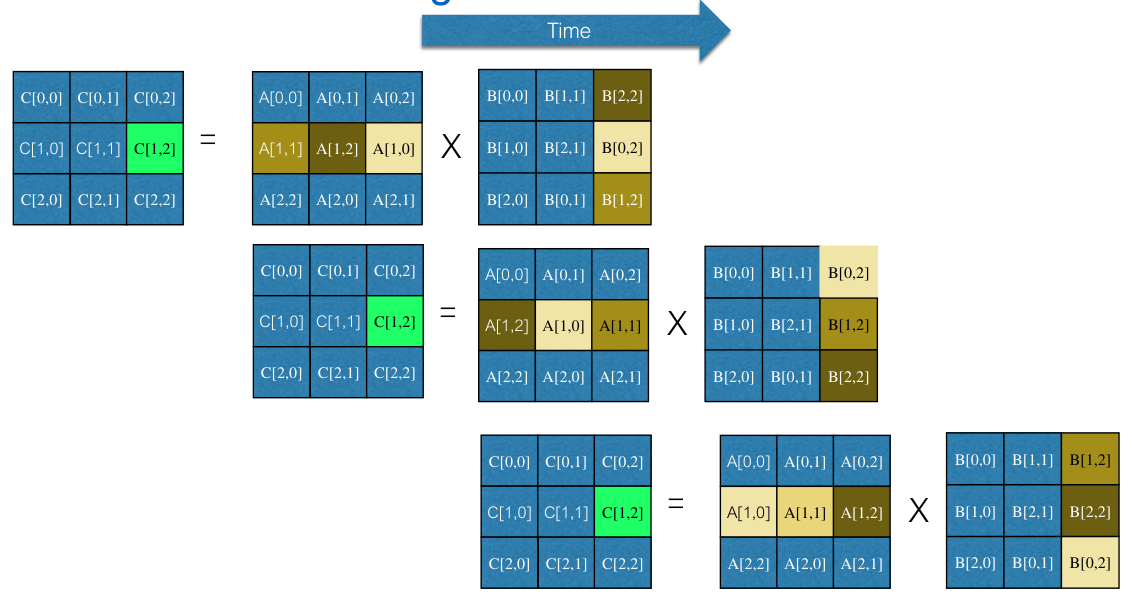
\includegraphics[width=2in]{images/cannon.jpg}
  \end{center}
  $T_p = 2\gamma\frac{n^3}{p} + 2 (1 + \sqrt{p})(\alpha + \beta\frac{n^2}{p})$

  $E_p = \frac{T_1}{pT_p}$ where $T_1 = 2n^3\gamma$

  Bounds when varying the size of $M$ is the size of the fast memory -- in this
  case the size of a per process tile.

  $T_p = \gamma \times \text{flop/s} + (\alpha \times
  \frac{\text{flop/s}}{M^{\frac{3}{2}}}) + (\beta^{-1}_\infty \times
  \frac{\text{flop/s}}{\sqrt{M}})$
  
  note that $\gamma$ is computing speed

  Communication avoidance: Cannon  overall does not reduce the amount of
  communication each proc sends 2 matricies $\frac{n^2}{p}$ to about $\sqrt{p}$
  procs. Just makes them more local and orderly. 

  Theoretical lower bound on communication 
  
  $ \# \text{words} = \Omega(\frac{\text{flop/s per proc}}{\sqrt{M}}) $ \&
  $ \# \text{messages} = \Omega(\frac{\text{flop/s per proc}}{M^{\frac{3}{2}}})$

  this follows for other linear algebra algs (LU, Cholesky, ...)


  Optimally with $M = \frac{n^2}{p}$: 
  $T_p = 2\gamma\frac{n^3}{p} + 2(1+\sqrt{p})(\alpha + \frac{\beta^{-1}n^2}{p})$
  

  Johnson’s 3D algorithm
  \begin{center}
    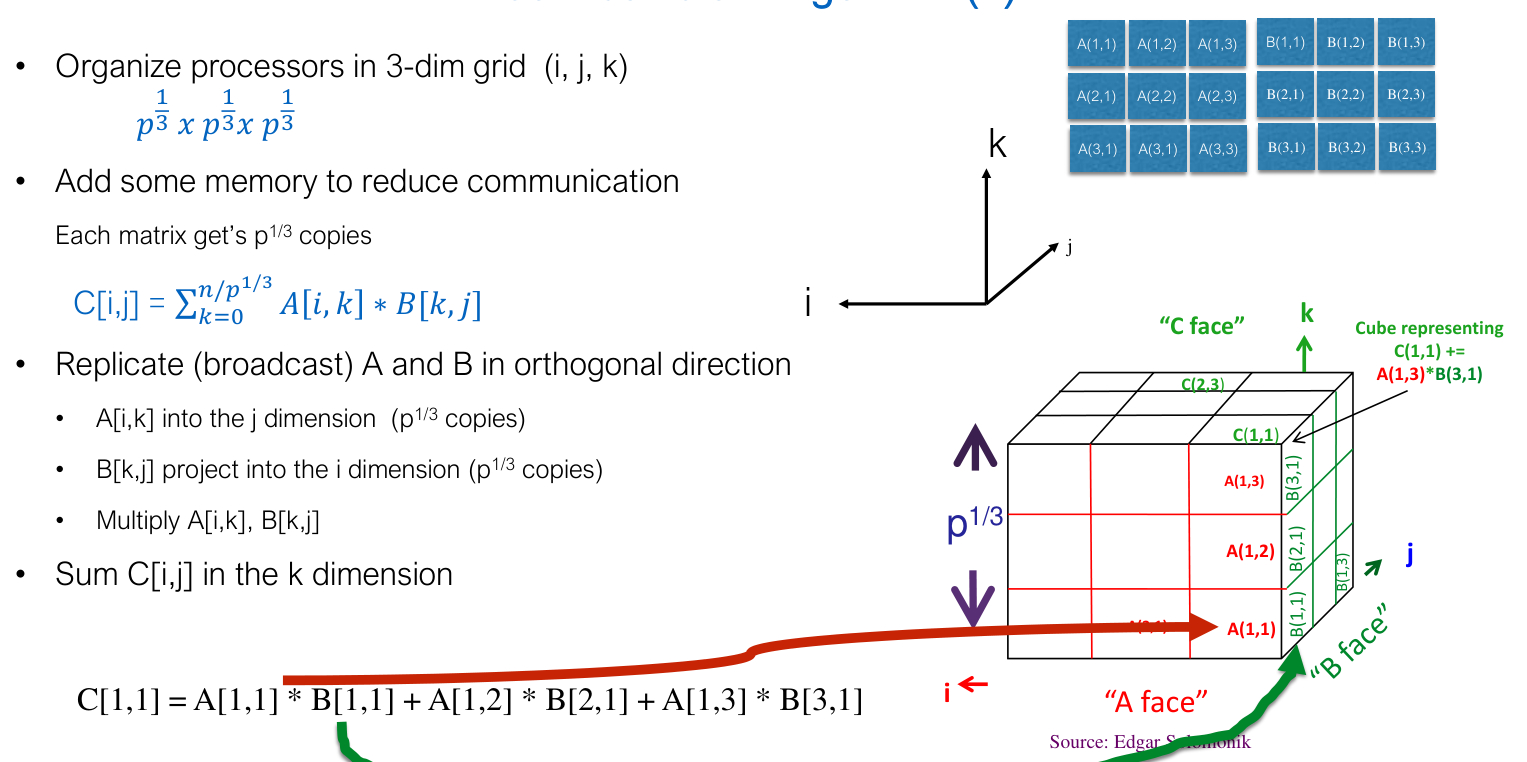
\includegraphics[width=2in]{images/johnson.jpg}
  \end{center}
  $M = O(\frac{n^2}{p^{\frac{2}{3}}})$, each process computes
  $O(\frac{n^2}{p^{\frac{2}{3}}})$ words. lower bound for bandwidth is
  $O(\frac{n^2}{p^{\frac{2}{3}}})$. and message latency is
  $O(\frac{n^3}{(\frac{n^2}{p^{\frac{2}{3}}})^{\frac{2}{3}}})$

  2.5D algorithm - Ballard and Demmel:  massively reduces communication and idl
  time
  \begin{center}
    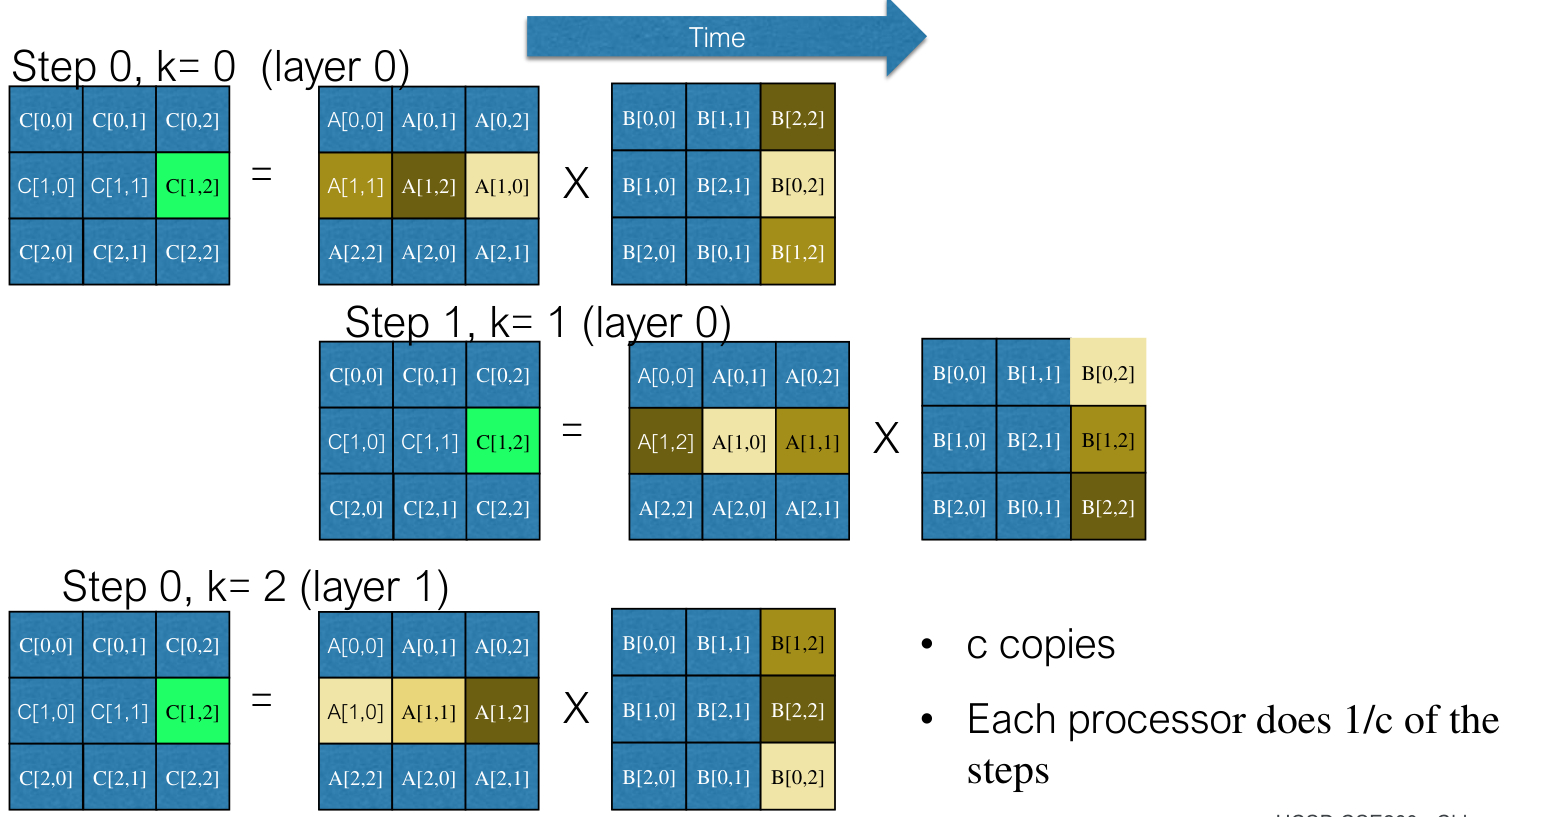
\includegraphics[height=1in]{images/2-5d-circular.jpg}
    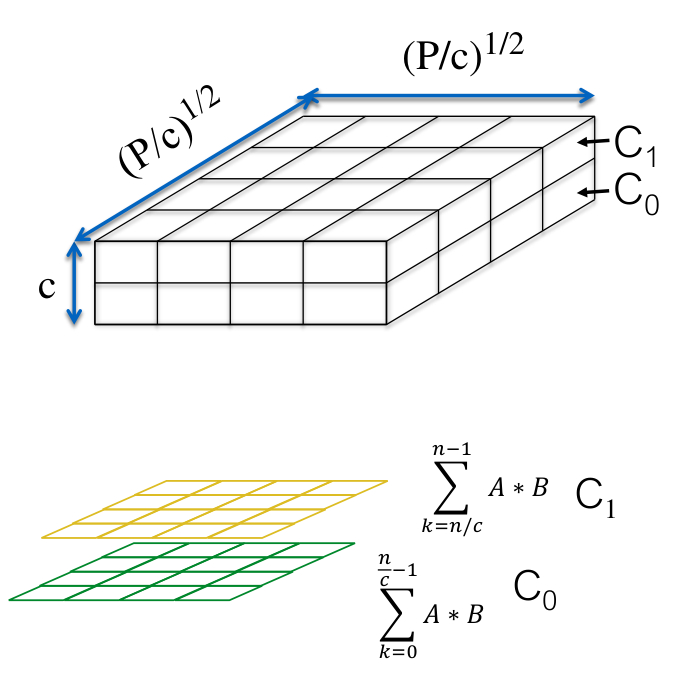
\includegraphics[height=1in]{images/2-5d-grid.jpg}
    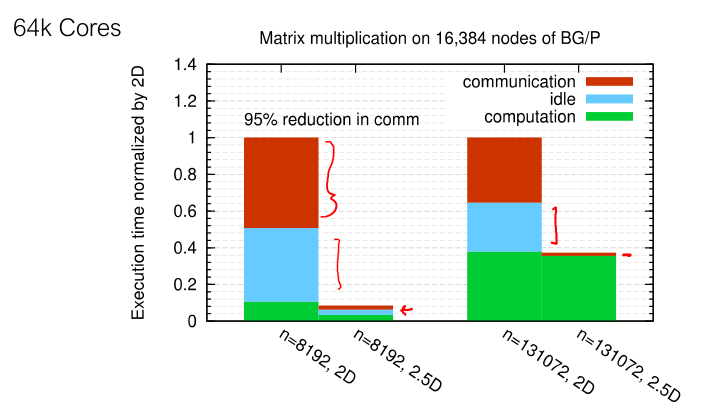
\includegraphics[height=1in]{images/2-5d-big.jpg}
  \end{center}

  have 2d cannon algorithm. expand to 3rd dim by factor of $c$
  with each layer doing $\frac{1}{c}$ of original cannon. sum layers to get
  final result. $\frac{cn^2}{p}$ data per proc. New grid is $\sqrt{\frac{p}{c}}
  \times \sqrt{\frac{p}{c}}\times c$. eg. $p=32 \implies c=2$. each Layer will
  only perform $\frac{k}{c}$ of the shifts with intial conditions being offsets
  of each other. $c$ copies of $A \& B$. performs
  $\frac{\sqrt{p}}{c^\frac{3}{2}}$ cannon steps for each copy of $A \& B$.
  reduce over $c$ layers of $C$. banwidth scaling: $O or \Omega
  (\frac{n^2}{\sqrt{cp}})$. Message scaling: cannon steps + reduction = 
  $O(\frac{\sqrt{p}}{c^{\frac{3}{2}}})$

  \section{SIMD}

  Vectorization: x86 has fixed simd instruction vectors while arm specifies
  variable length vector registers from 128 up to 2048 bit vectors  (size of
  vectors is dependant on whoever is implementing the arm core. ARM SVE allows for
  predication to deal with tail cases. predicate is set with FFR (first faulting
  register) to check if bounds have been hit with SVE vector.

  Strip mining: Given a vector machine with a fixed vector length break down for
  loops such that some of the inner loops are of fixed length to be vectorized
  for instruction level parallel. For gpus this exists as warp dispatch which
  exists under the hood abstracted away from programmer.

  Control divergence: when threads in the same warp diverge into different
  instruction paths. Can cause reissuing of warp to follow said different
  control path. Will result in some lanes being disabled and reissued to follow
  unfollowed control path.

  Loop carried dependencies: an iteration of a loop depends on another
  iteration.

  \section{Multithreading}

  OpenMP: exists as a series of compiler directed for easy spawning of threads
  on loops where the requirement is loops need to not possess any loop carried
  dependencies. openMP is not smart and will parallelize into data races if done
  poorly. 

  True dependencies: between two instructions the input of one depends on the
  output of another

  Output dependencies: between two instructions both are writing to a variable
  so, end value of variable is indeterminant if done in parallel

  Anti dependencies: if a preceding instruction requires a value that will be
  overwritten later. 

  Barriers: openmP will create implicit barriers after exiting each parallel
  directive.

  atomics:\verb|#pragma omp atomic| 

  mutex: \verb|#pragma critical|

  OpenMP reductions: handles atomicity and synctronization -- need to specify
  value being reduced to \verb|#pragma omp parallel reduction (+:varname)|

  \section{Gpu Architecture}

  cuda:

  GPU Memory Hierarchy:
  \begin{center}
    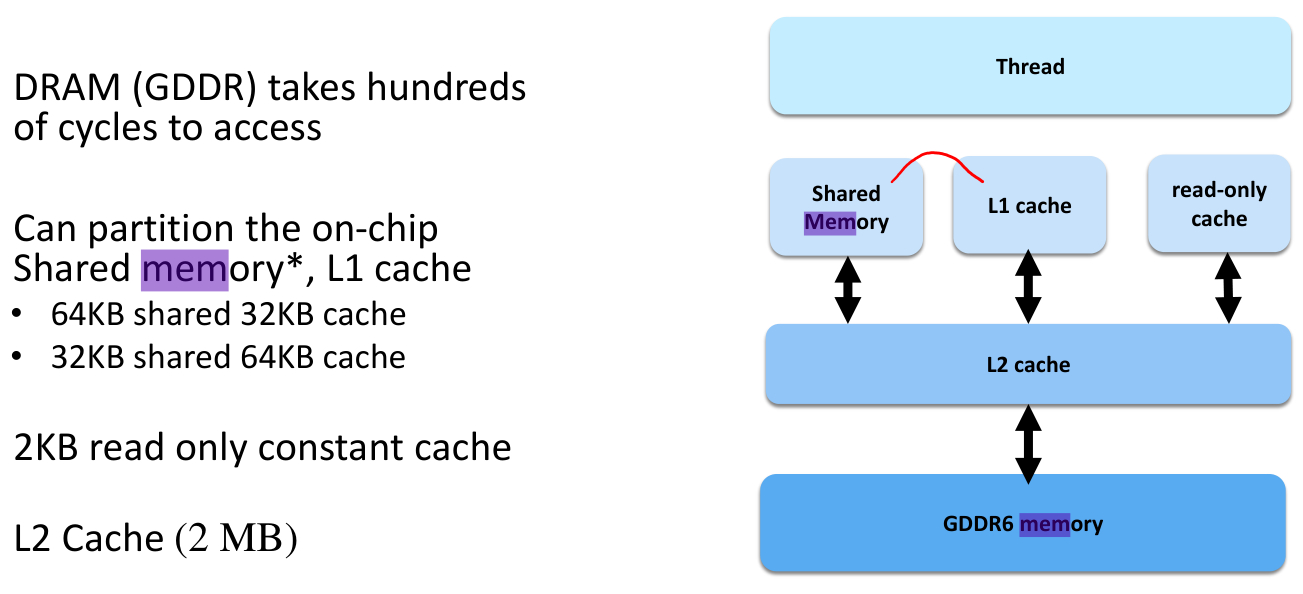
\includegraphics[width=2in]{images/gpu-mem.jpg}
  \end{center}

  GPU Thread Hierarchy: threads grouped into threadblocks. threadblocks are
  minimum dispatch units for a kernel and are allocated to streaming
  multiprocesessors. Grids are multiple such blocks and a kernel is executed on
  a grid. 

  GPU warp scheduling: $\text{thread} \subset \text{warp} \subset\text{thread block} \subset\text{grid}$

  \begin{center}
    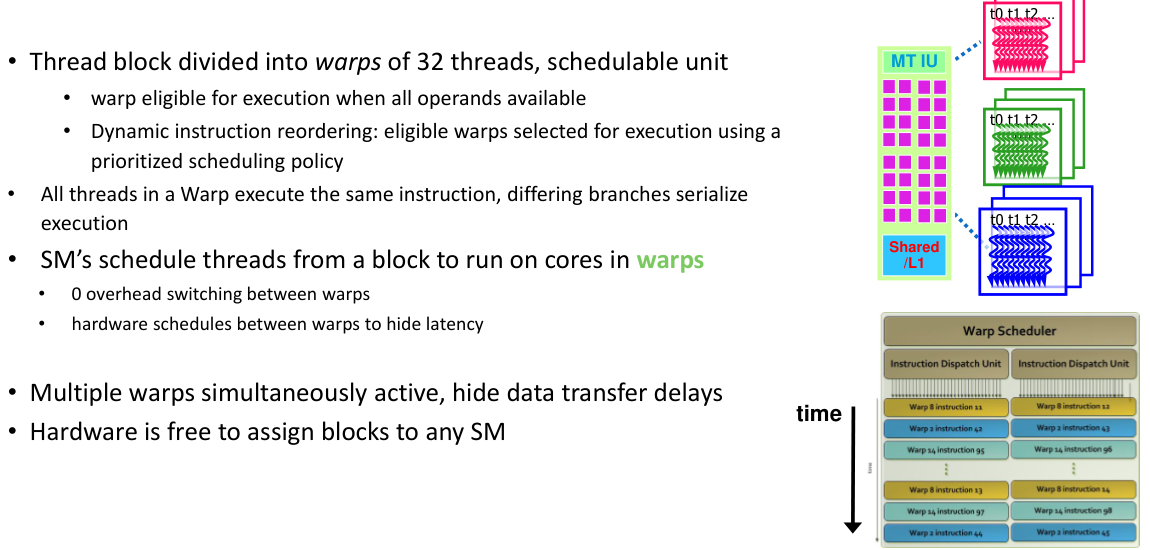
\includegraphics[width=2in]{images/warp-scheduling.jpg}
    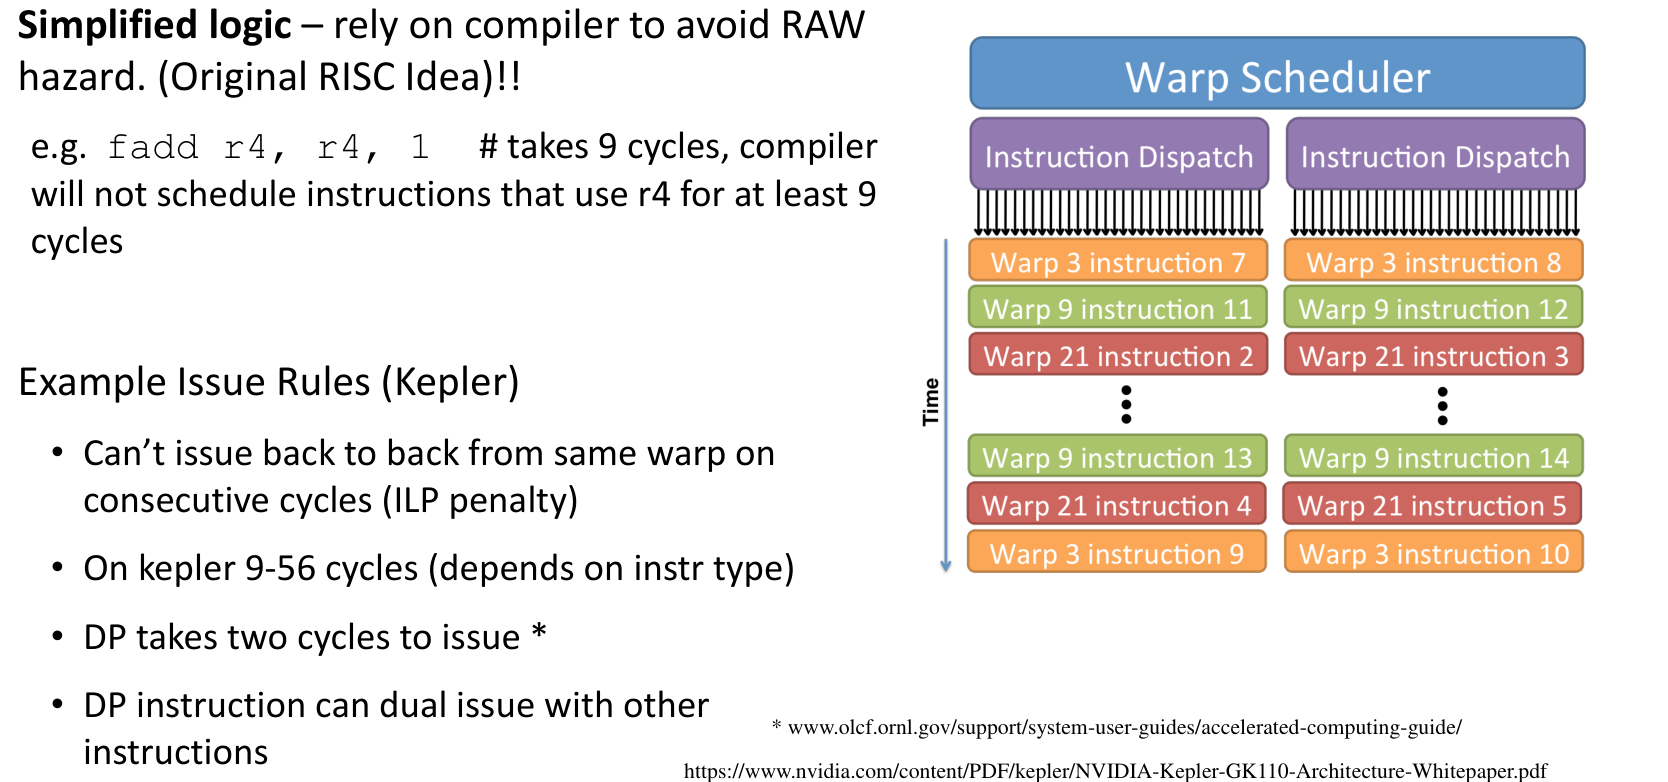
\includegraphics[width=2in]{images/warp-scheduling2.jpg}
  \end{center}

  GPU thread mapping to warps
  \begin{center}
    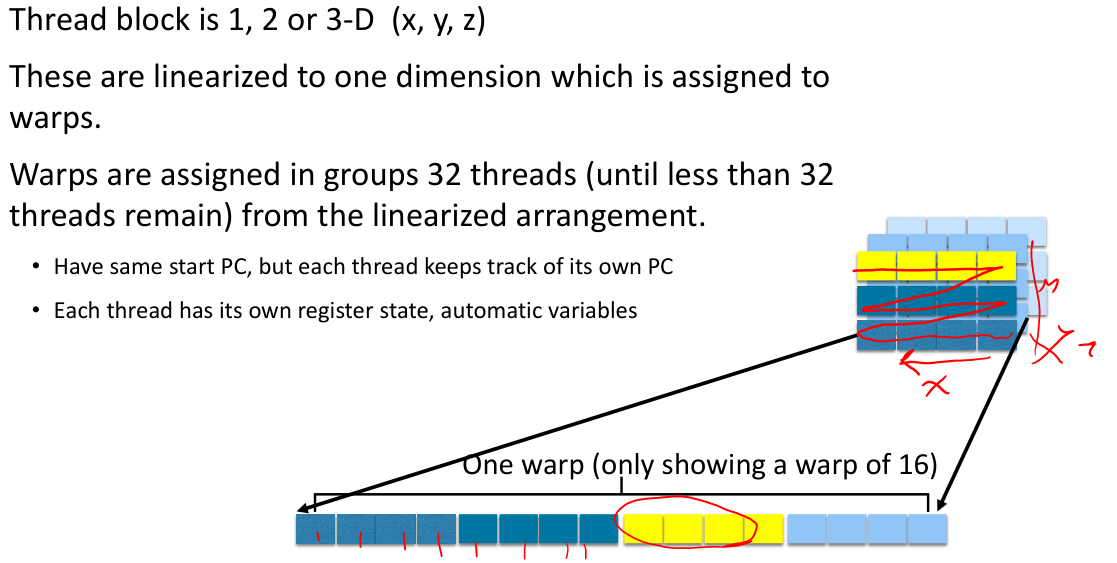
\includegraphics[width=2in]{images/thread-mapping-warp.jpg}
  \end{center}

  Comp intensity naive on gpu: $q = \frac{2n^3}{2n^3 + 2n^2}$, $2n^2$ load and
  stores from $C$. $2n^3$ loads from $A\&B$

  Matrix Multiply on GPU – techniques (e.g. tiling): its dumb look at pa2. A lot of syncing threads is needed between loading shit in and performing
  computation on it

  Estimated speedup from tiling: fuck if i know like 2x?

  Parallel Speedup computation: big $n$

  Occupancy = $\frac{\text{\# active warps}}{\text{max warps per M}}$.
  occupancy can hint at register/share memory usage, on a per warp basis along
  with thread register usage.

  Cusp behavior – TLP and ILP: use o filp will increase bw slope and hid latency
  with ilp. 
  $O_{cc} = \text{latency} \times \min(\text{mem throughput},
  \frac{alu_{thru}}{\alpha}, \frac{alu_{issue_{thru}}}{\alpha + 1})$. where
  latency $= (mem_{lat} + \alpha \times alu_{lat})$. as a result for small
  $\alpha$ (mem bound) $O_{cc} = mem_{lat}mem_{thru} + \alpha \times
  alu_{lat}mem_{thru}$. For large $\alpha$ (alu/issue bound): $O_{cc} =
  \frac{mem_{lat}alu{thru}}{\alpha} +  alu_{lat}alu_{thru}$. max required
  occpancy $= mem_{lat}mem_{thru} + alu_{lat}alu_{thru}$
  \begin{center}
    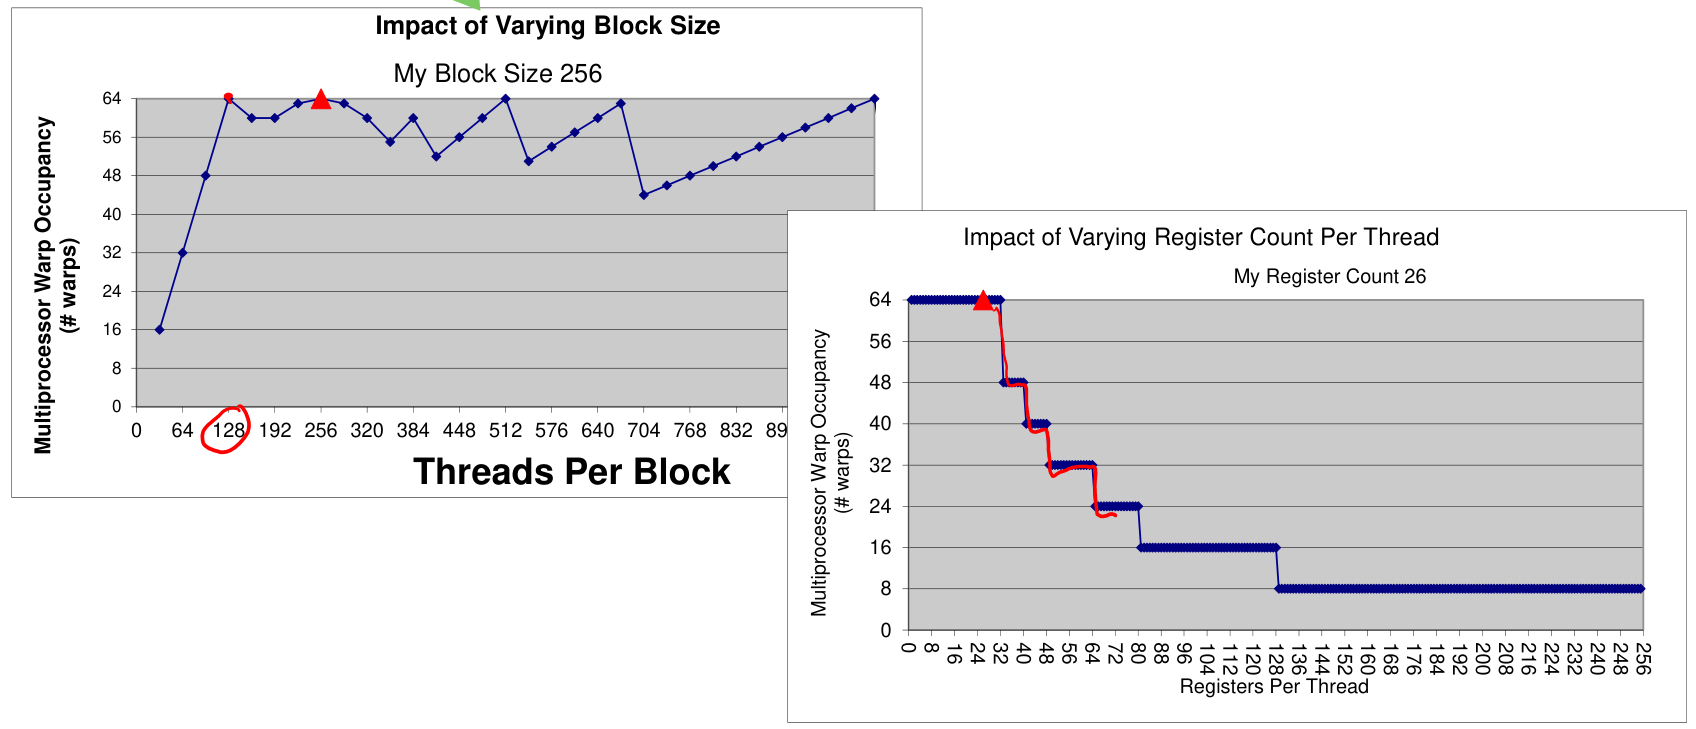
\includegraphics[width=2in]{images/occupancy-drop.jpg}
    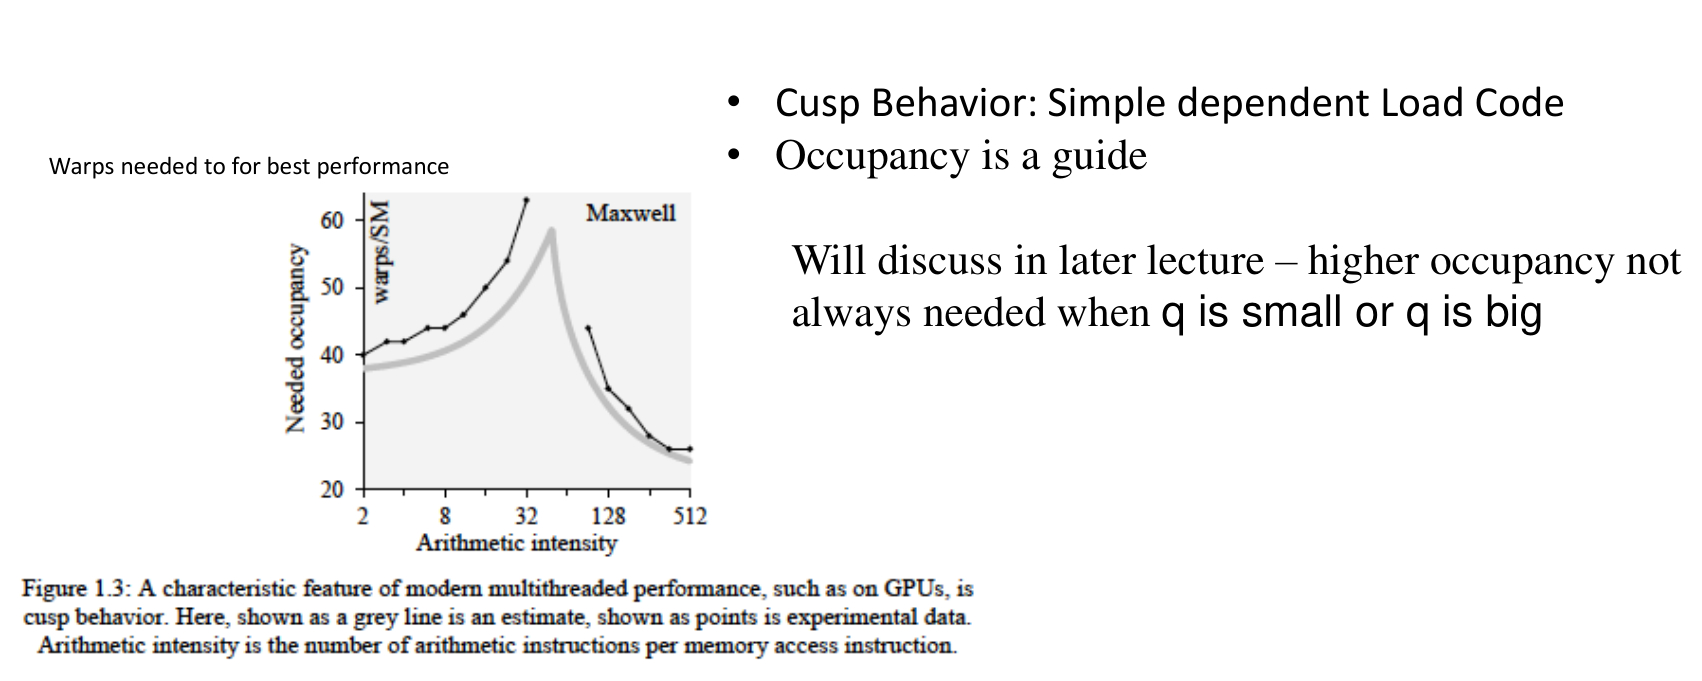
\includegraphics[width=2in]{images/cusp.jpg}
    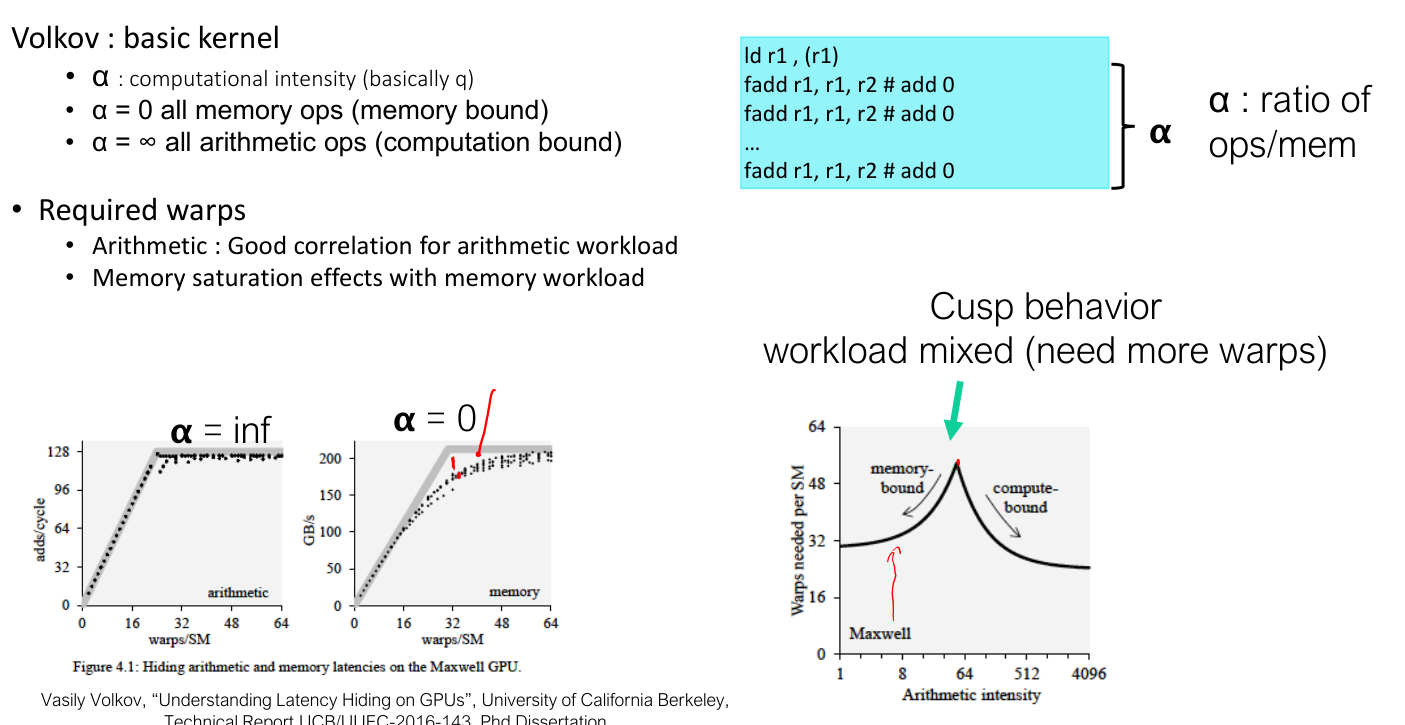
\includegraphics[width=2in]{images/gpu-hit-lat.jpg}
    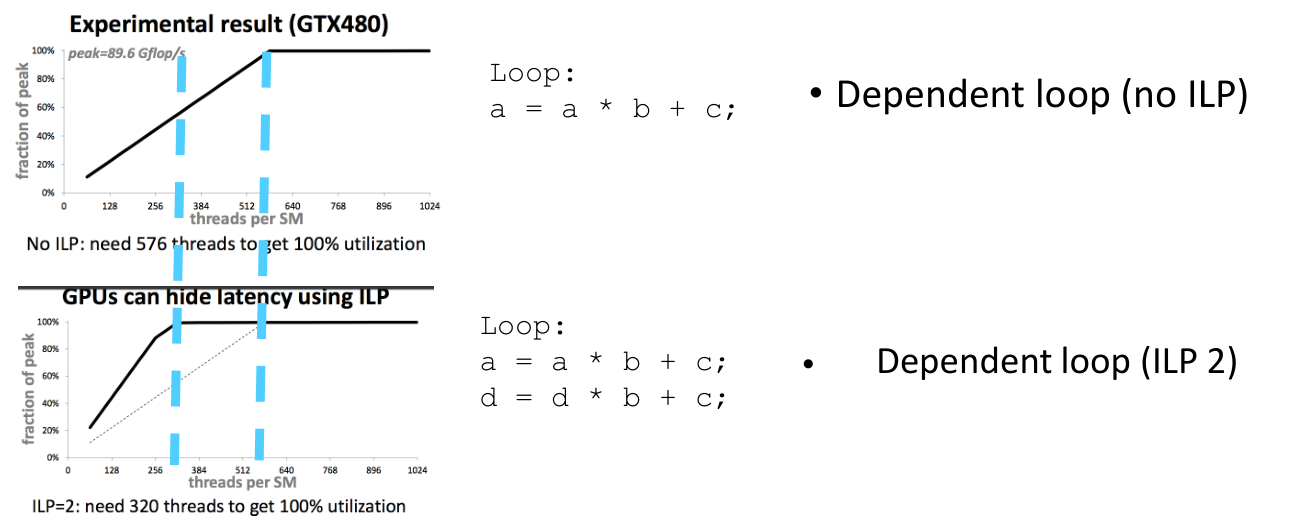
\includegraphics[width=2in]{images/ilp-thru.jpg}
  \end{center}

  GPU Memory Interleaving:
  \begin{center}
    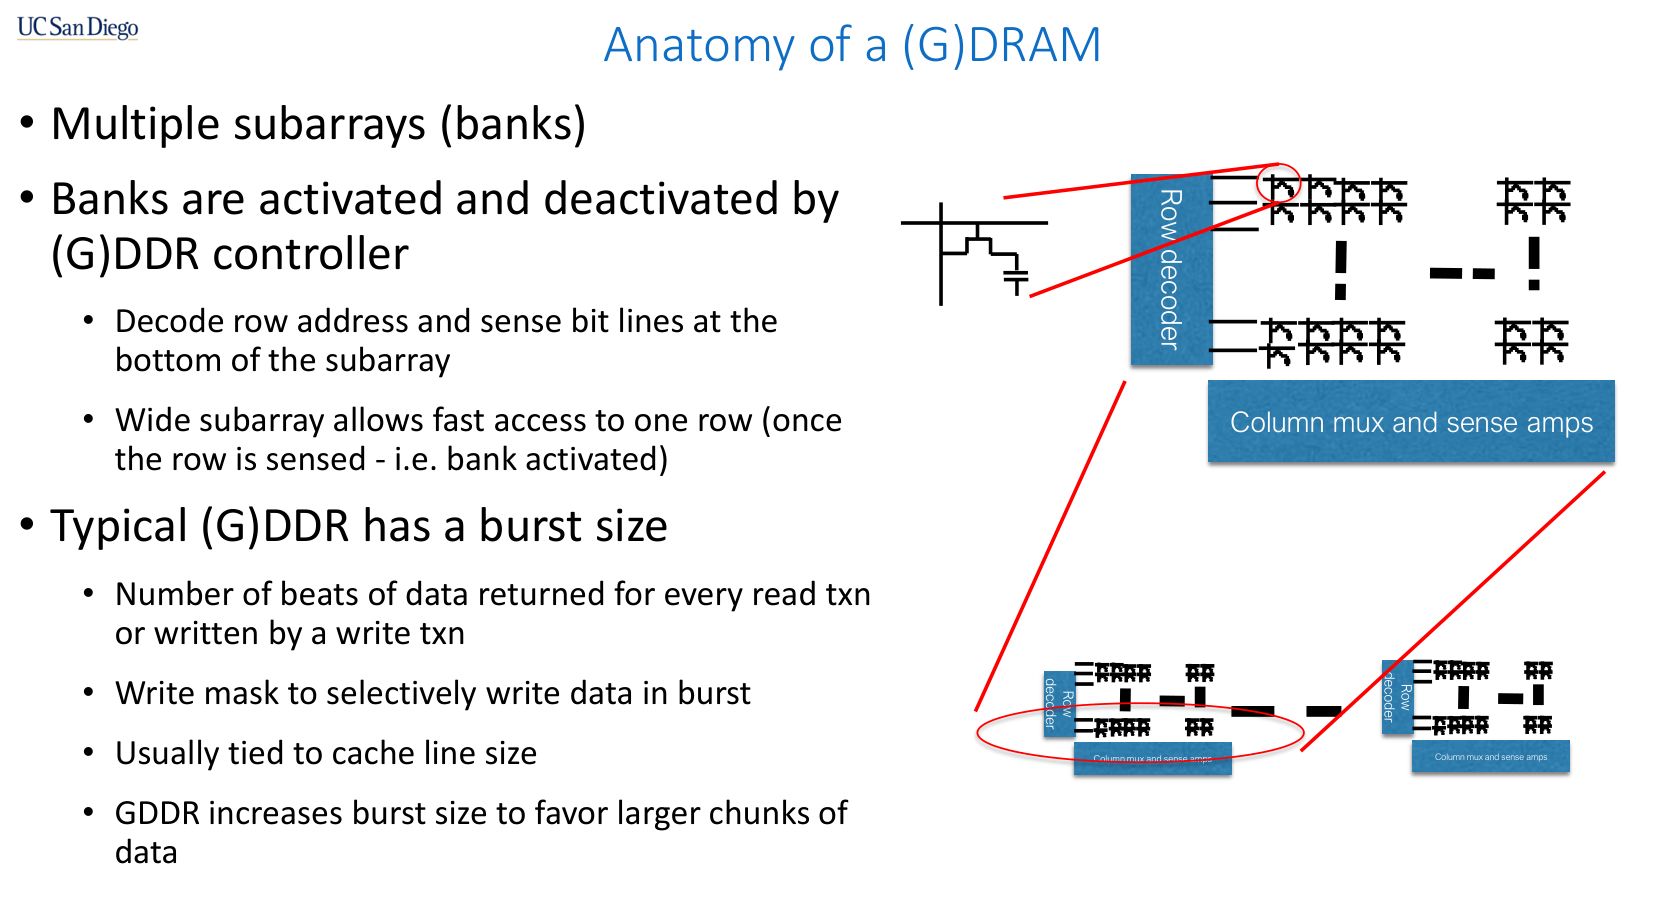
\includegraphics[width=2in]{images/gdram.jpg}
    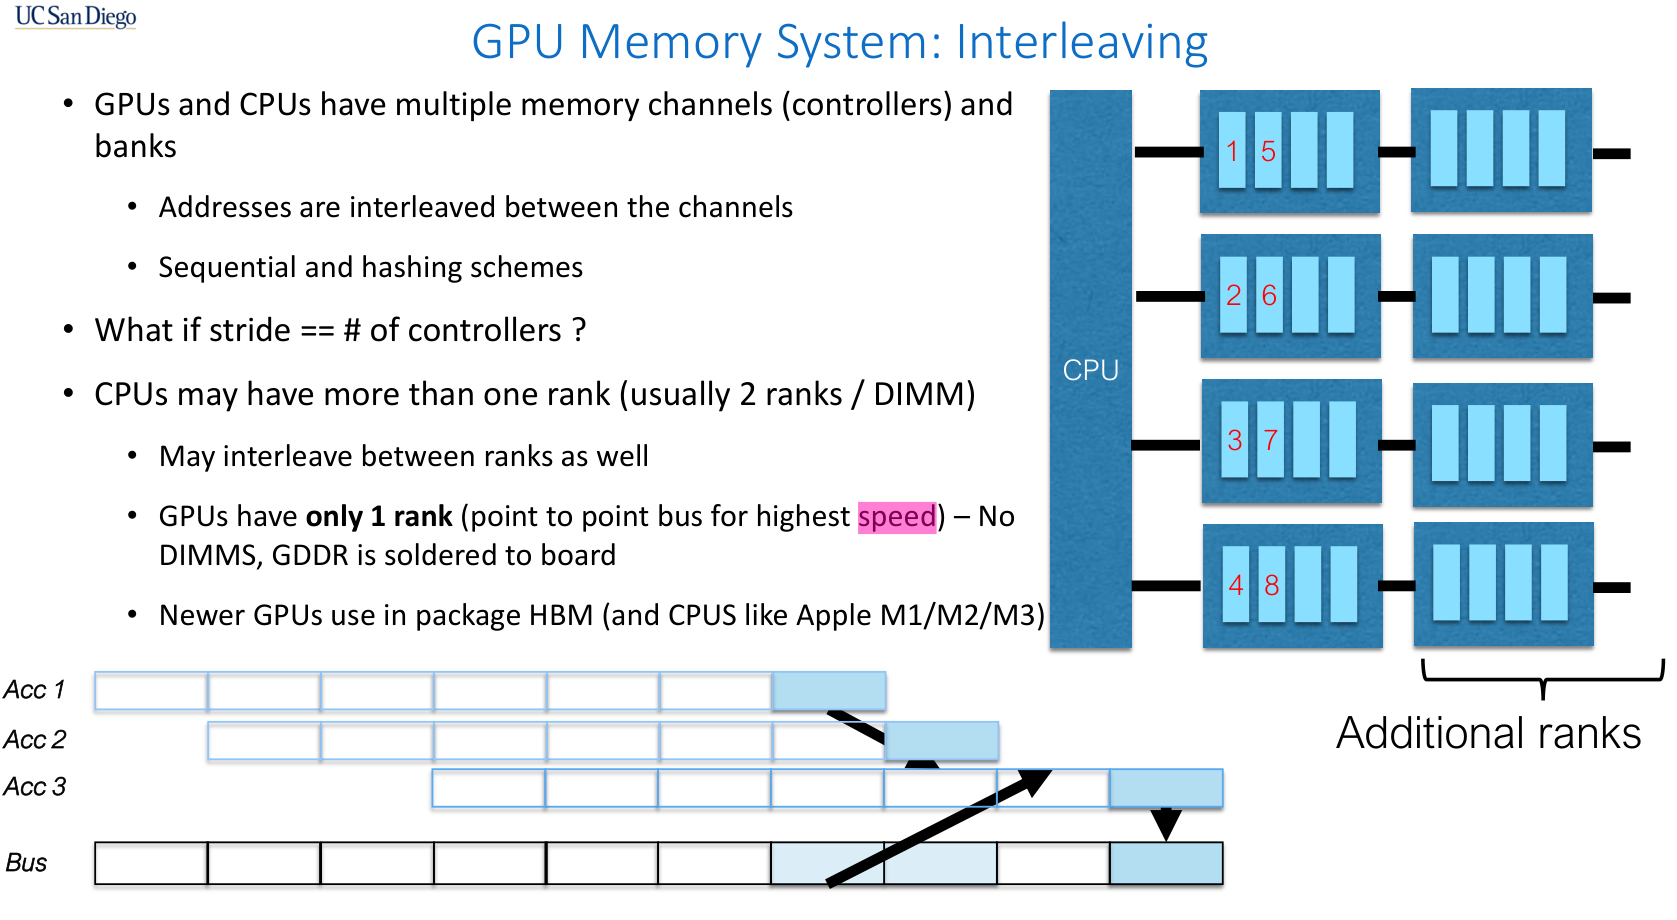
\includegraphics[width=2in]{images/interleaving.jpg}
  \end{center}

  GPU Memory Coalescing: access of a 32 bit aligned 4 byte word vector w/o bank
  conflicts -- tldr reduce loads by making loads be big.
  \begin{center}
    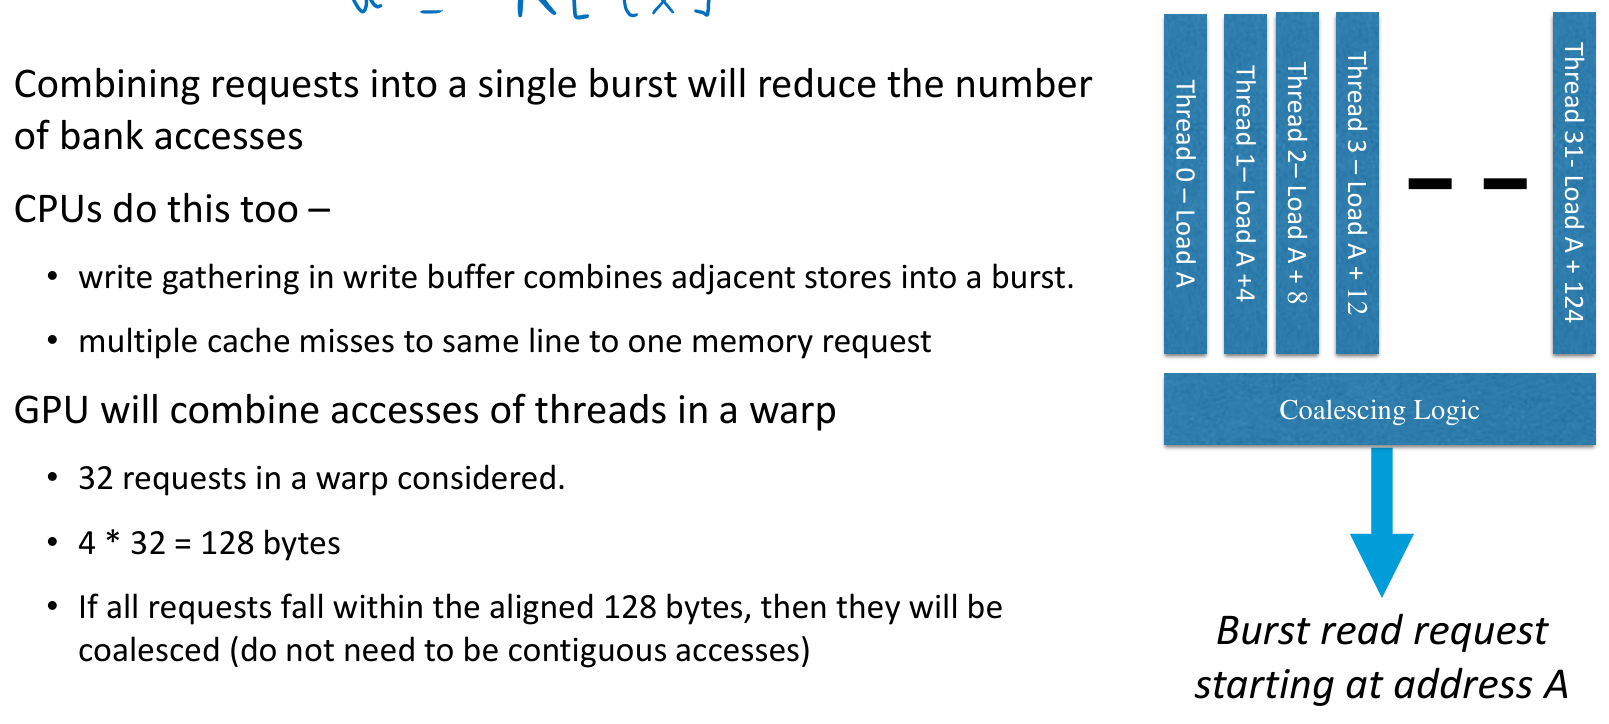
\includegraphics[width=2in]{images/coalescing.jpg}
  \end{center}

  GPU Bank access and bank conflict avoidance |
  \begin{center}
    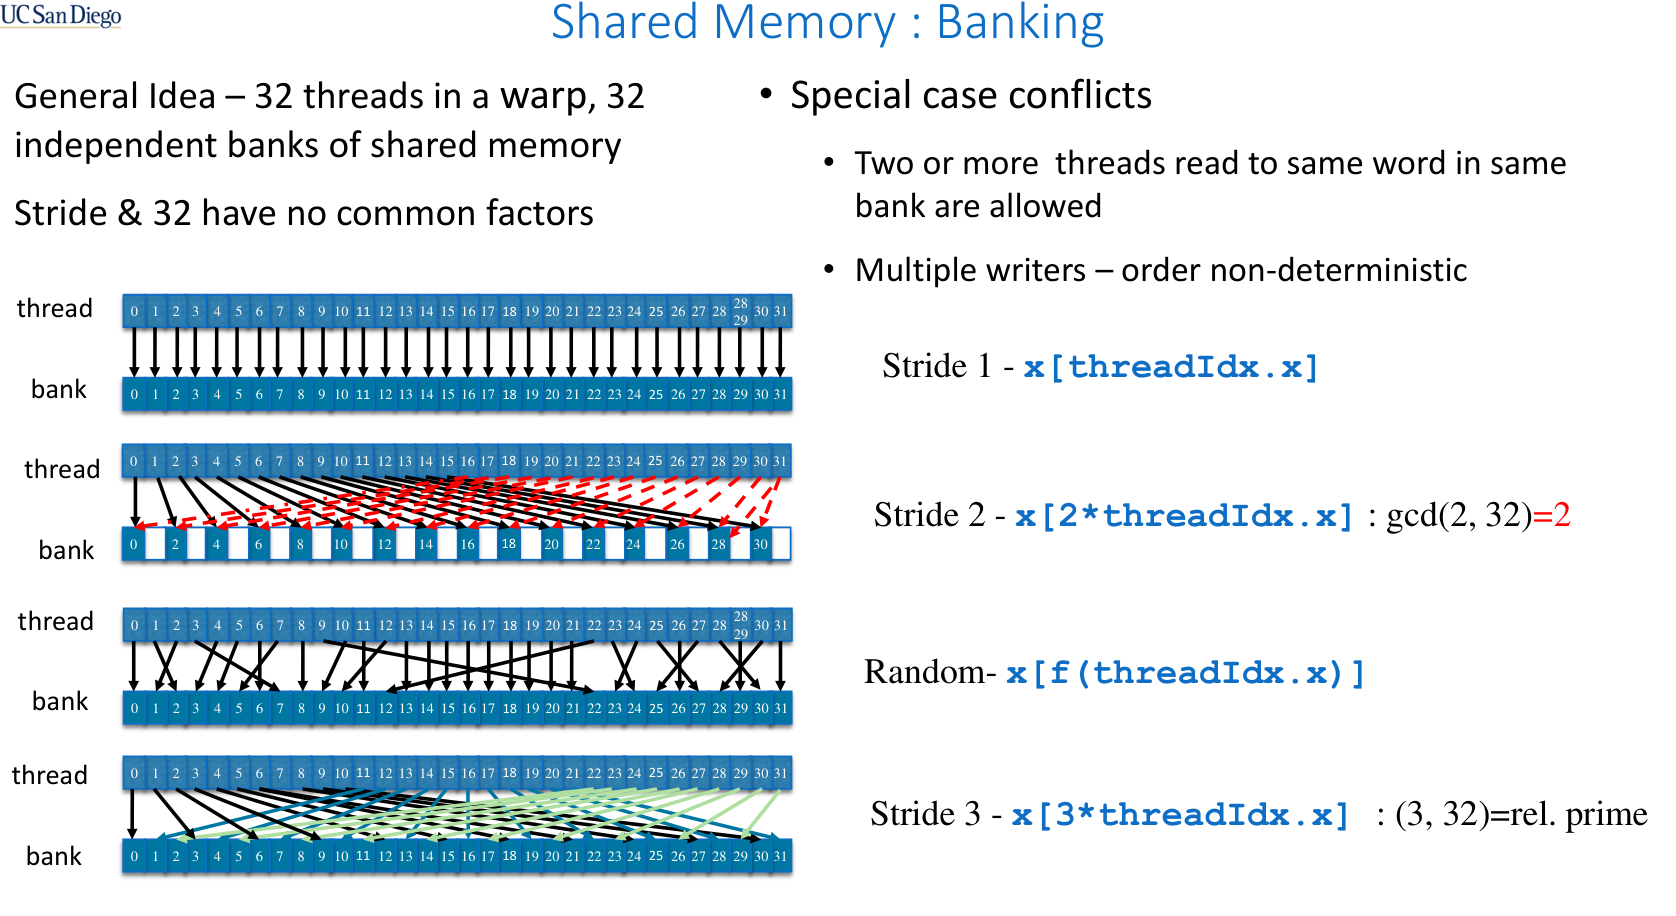
\includegraphics[width=2in]{images/banks.jpg}
  \end{center}
  
  Thread Level and Instruction Level Parallelism
  \begin{center}
    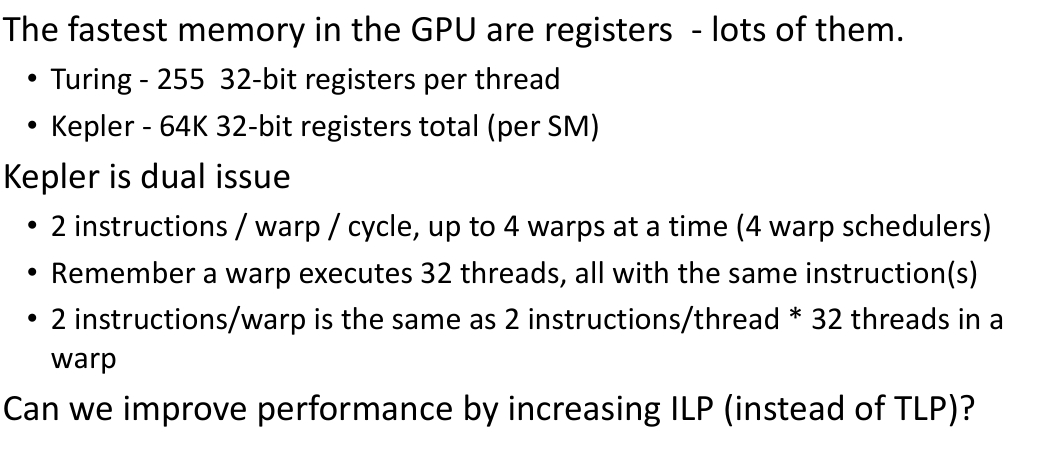
\includegraphics[width=2in]{images/gpu-ilp.jpg}
    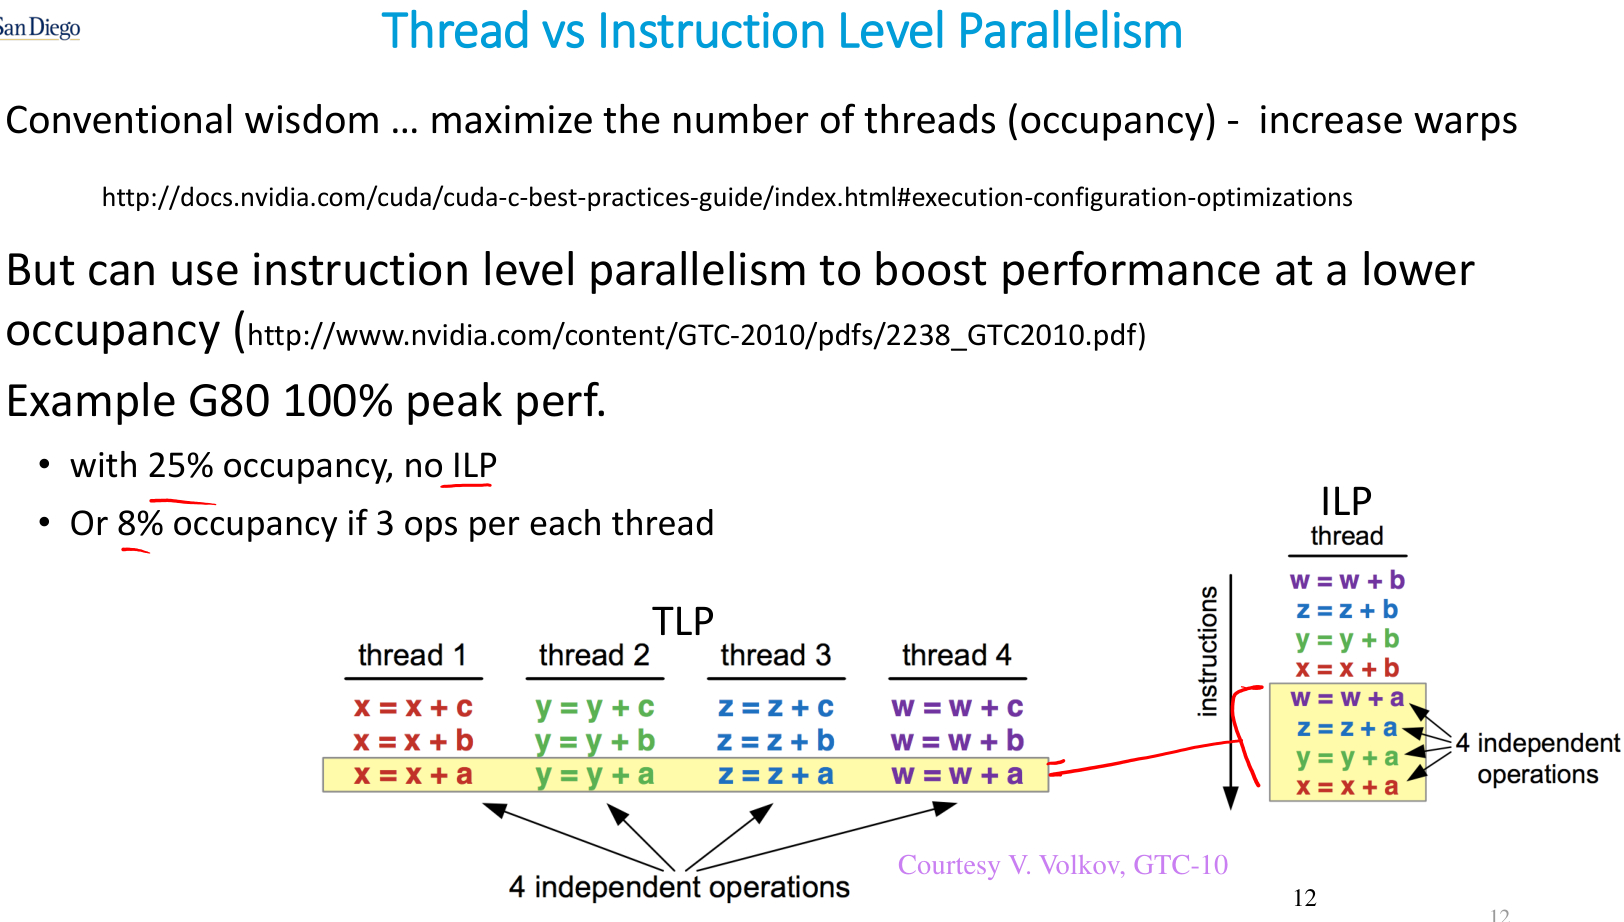
\includegraphics[width=2in]{images/gpu-tlp-ilp.jpg}
  \end{center}
  



  Little’s Law and GPUs |
  Concept of Arithmetic Latency and Memory Latency in GPUs |
  \begin{center}
    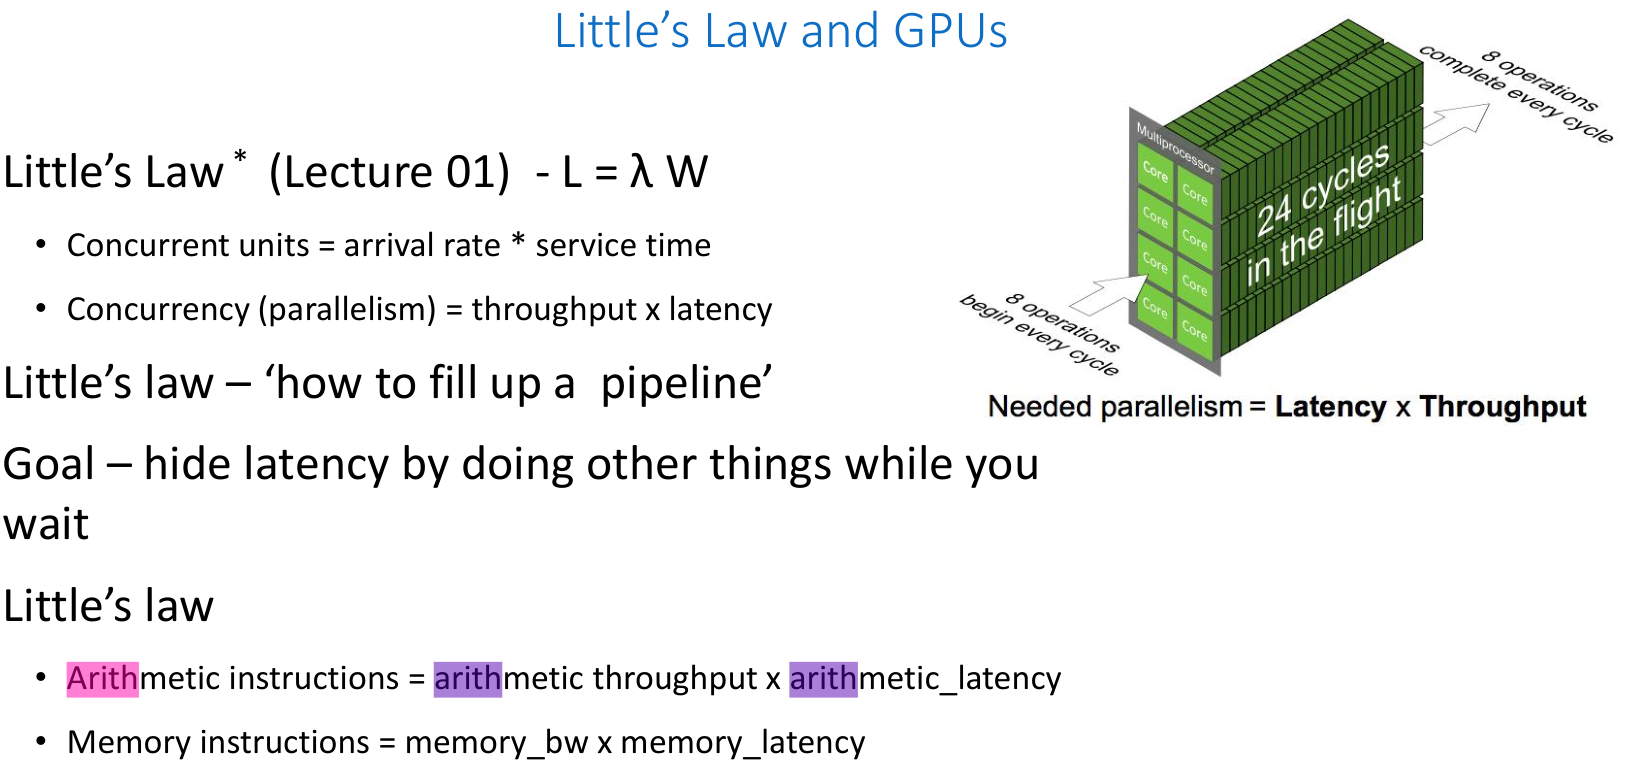
\includegraphics[width=2in]{images/gpu-little.jpg}
    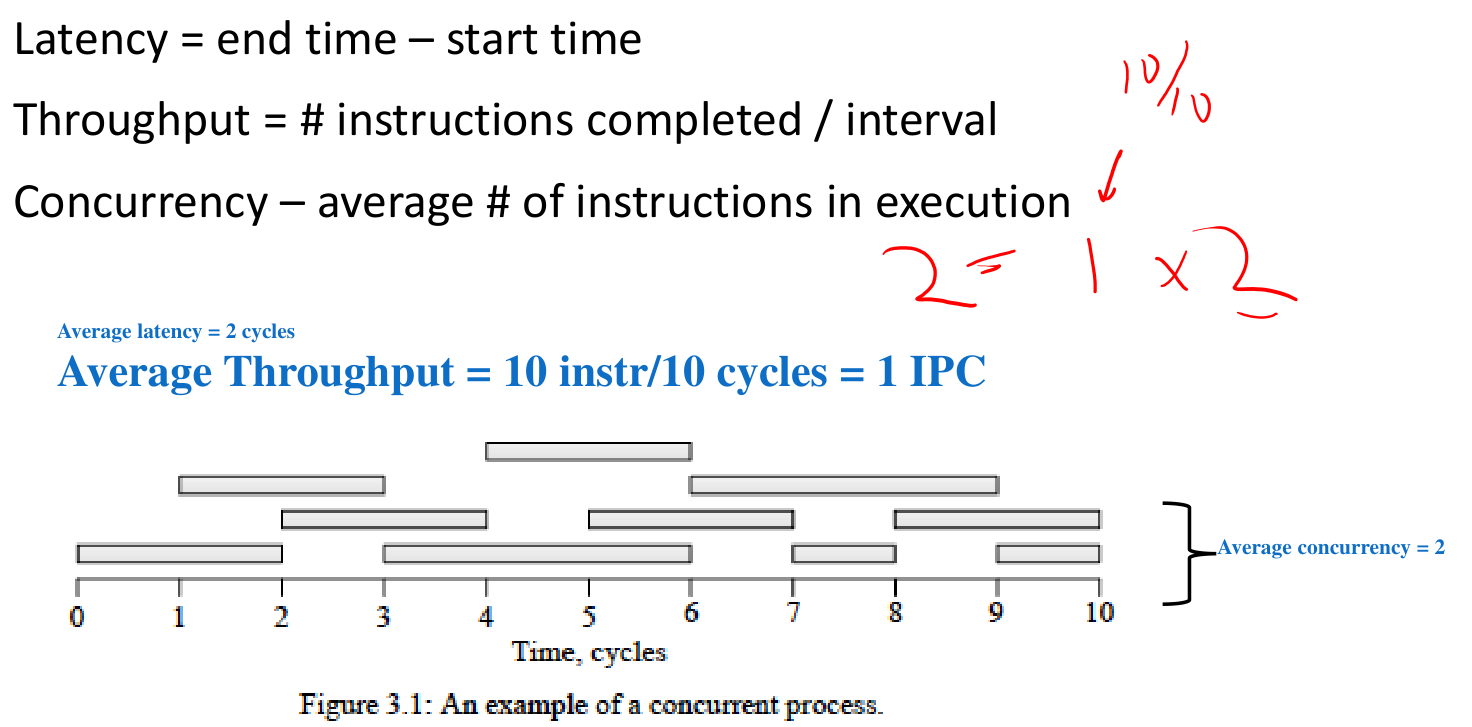
\includegraphics[width=2in]{images/gpu-ilp-little.jpg}
    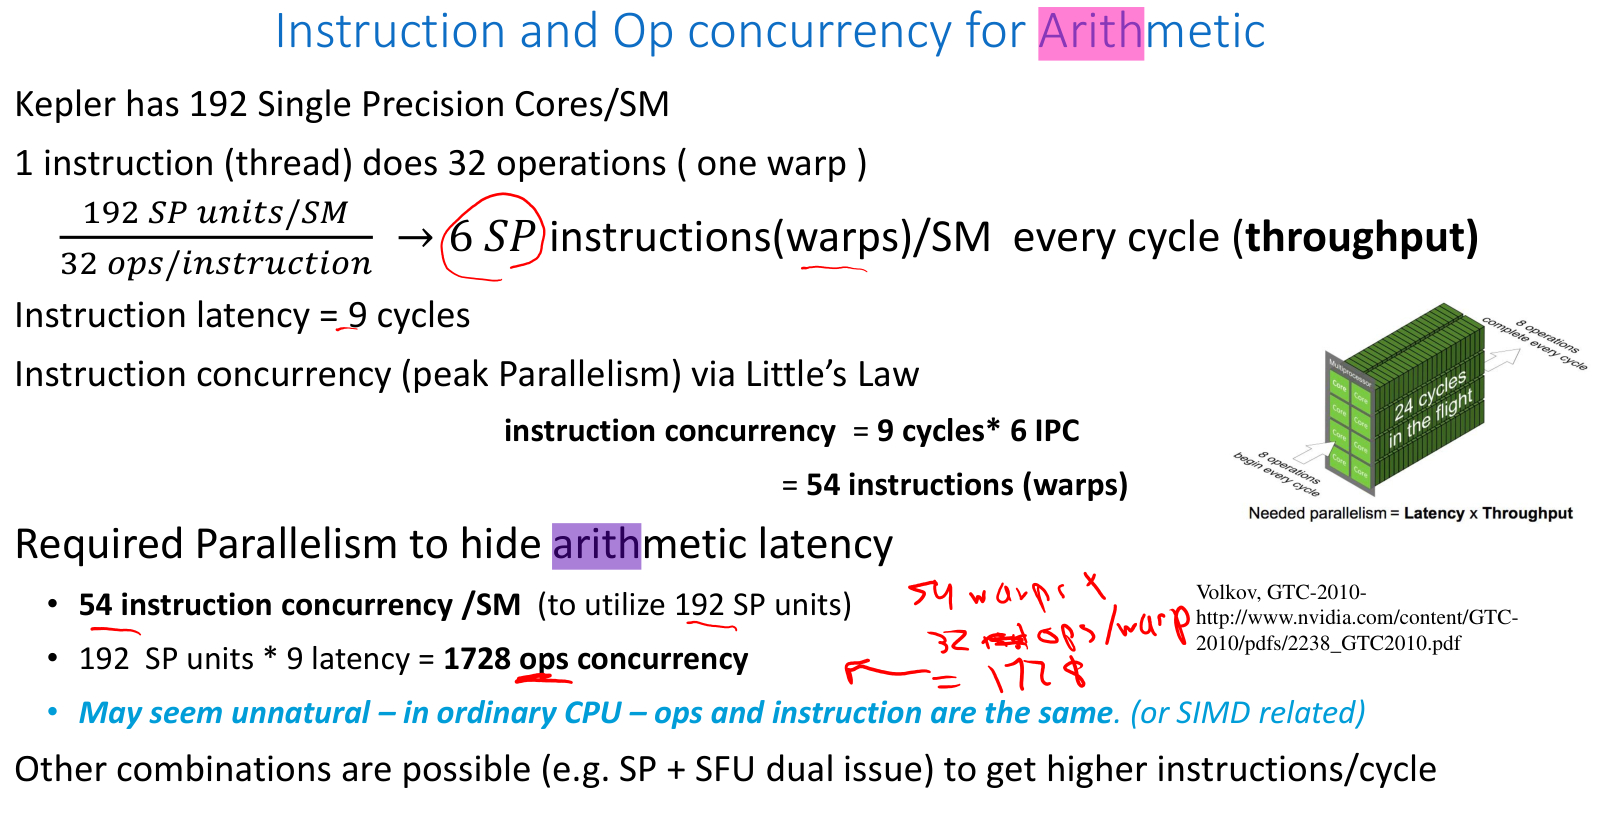
\includegraphics[width=2in]{images/gpu-ilp-eg.jpg}
    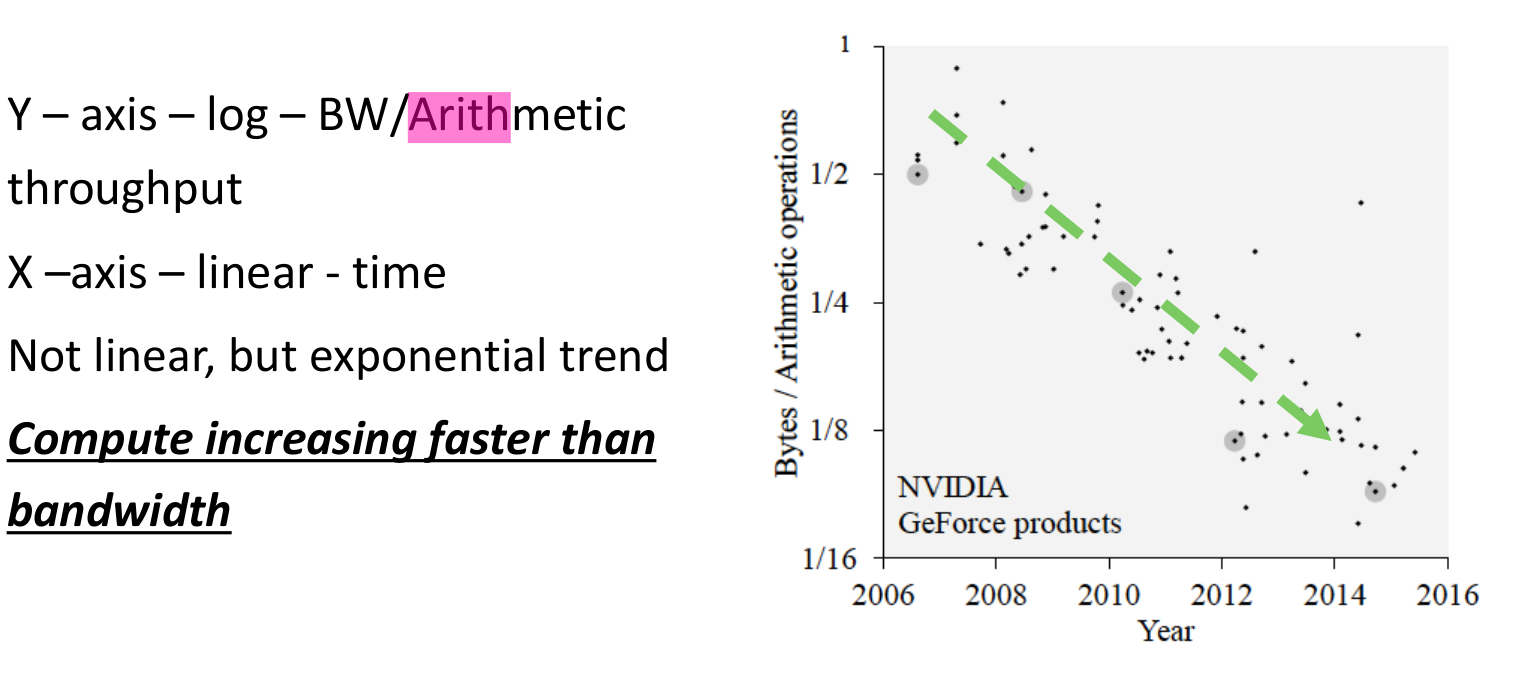
\includegraphics[width=2in]{images/mem-wall.jpg}
  \end{center}

  CUDA compilation flow to achieve source code portability between generations:
  shit doesnt exist or smth idk i give up
  (nvcc->ptx->ptxas->binary) |

  Predication vs. branching, thread divergence: Control divergence in a GPU
  shit exists on arm sve u did it for pa1 dont bother me
  Costs – why does it happen: reordering of kernel consider it a branch kinda
  miss -- since gpus don't really branch predict. smth smth flishing of pipeline

  Do all branches cause control divergence?: no only when it invokes a different
set of flow control -- branches can allow for values to be changed but if it
changes the control flow then it will diverge. note tho this will only occur on
a per warp basiss not a per thread basis. common to occur when conidition for is
on a threadid.
  \begin{center}
    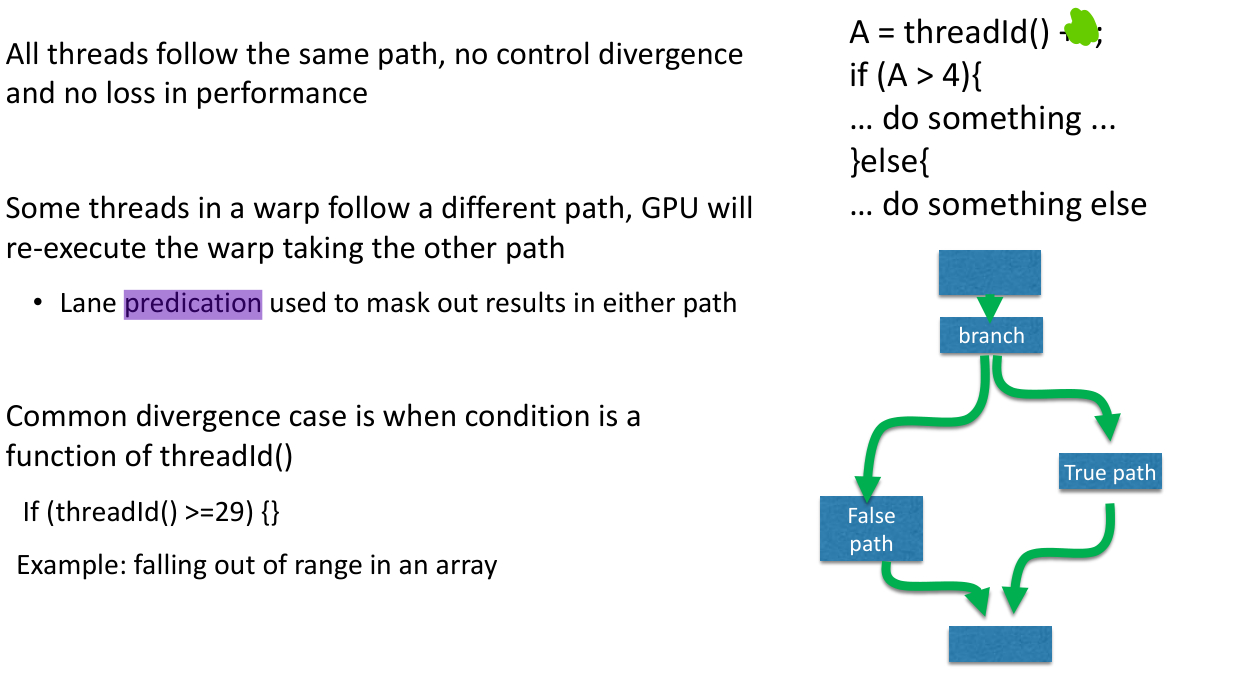
\includegraphics[width=2in]{images/gpu-predication.jpg}
    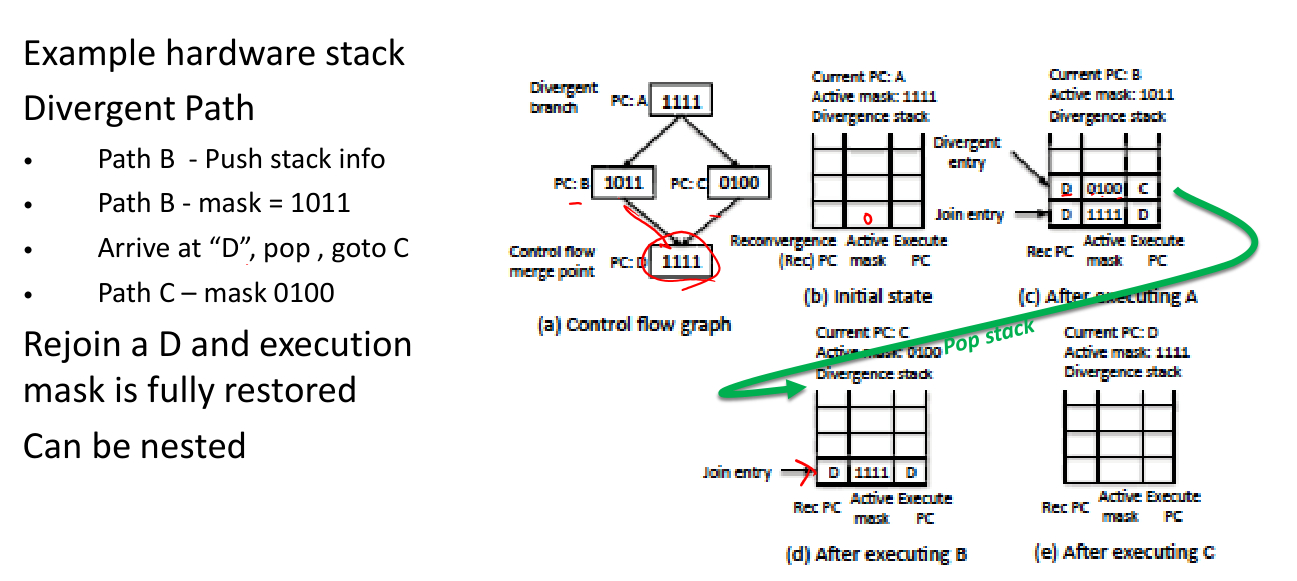
\includegraphics[width=2in]{images/gpu-divergence.jpg}
    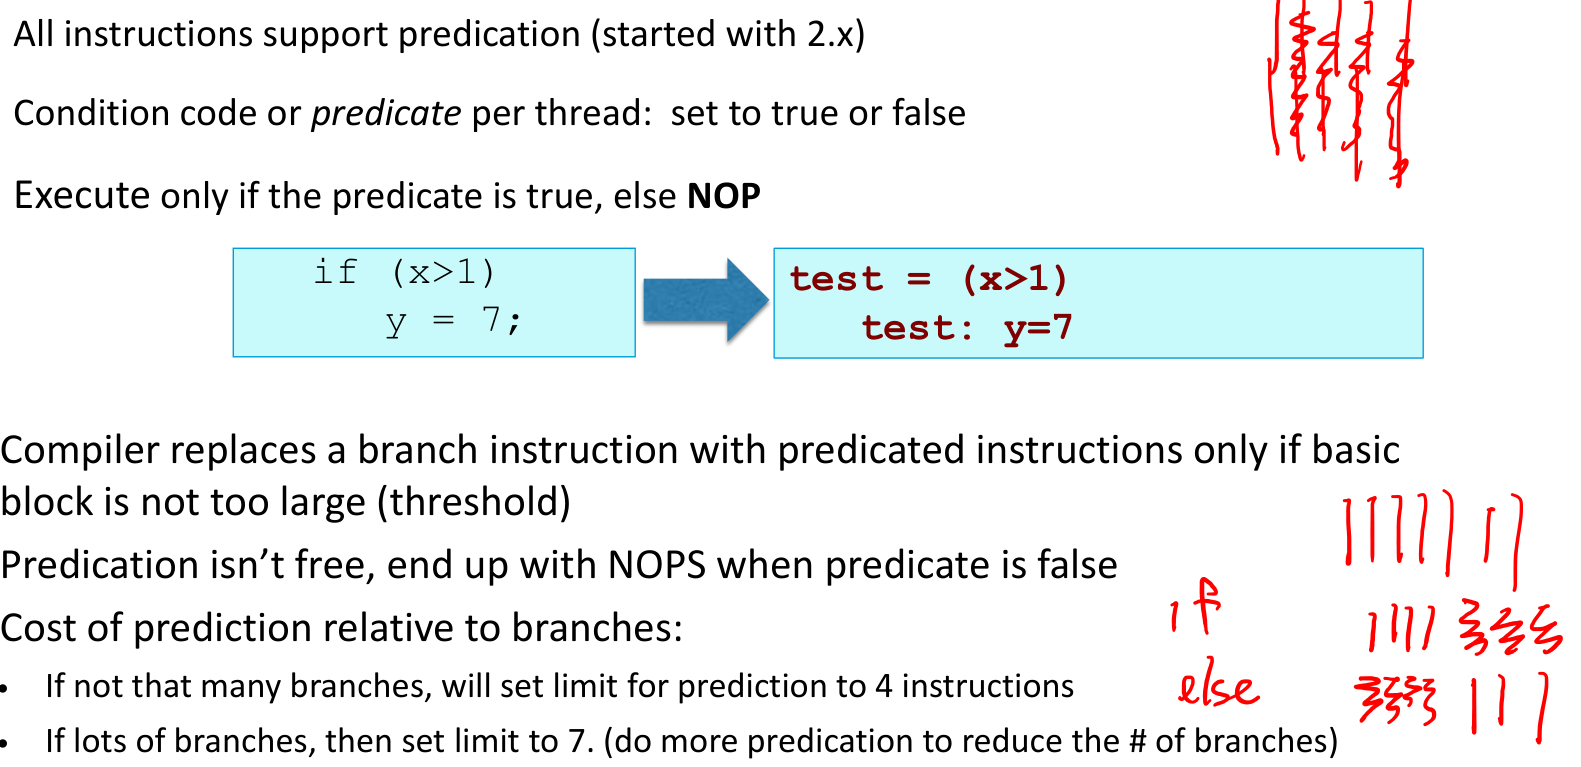
\includegraphics[width=2in]{images/cuda-predication.jpg}
  \end{center}

  Stripmining in the context of GPUs
  \begin{center}
    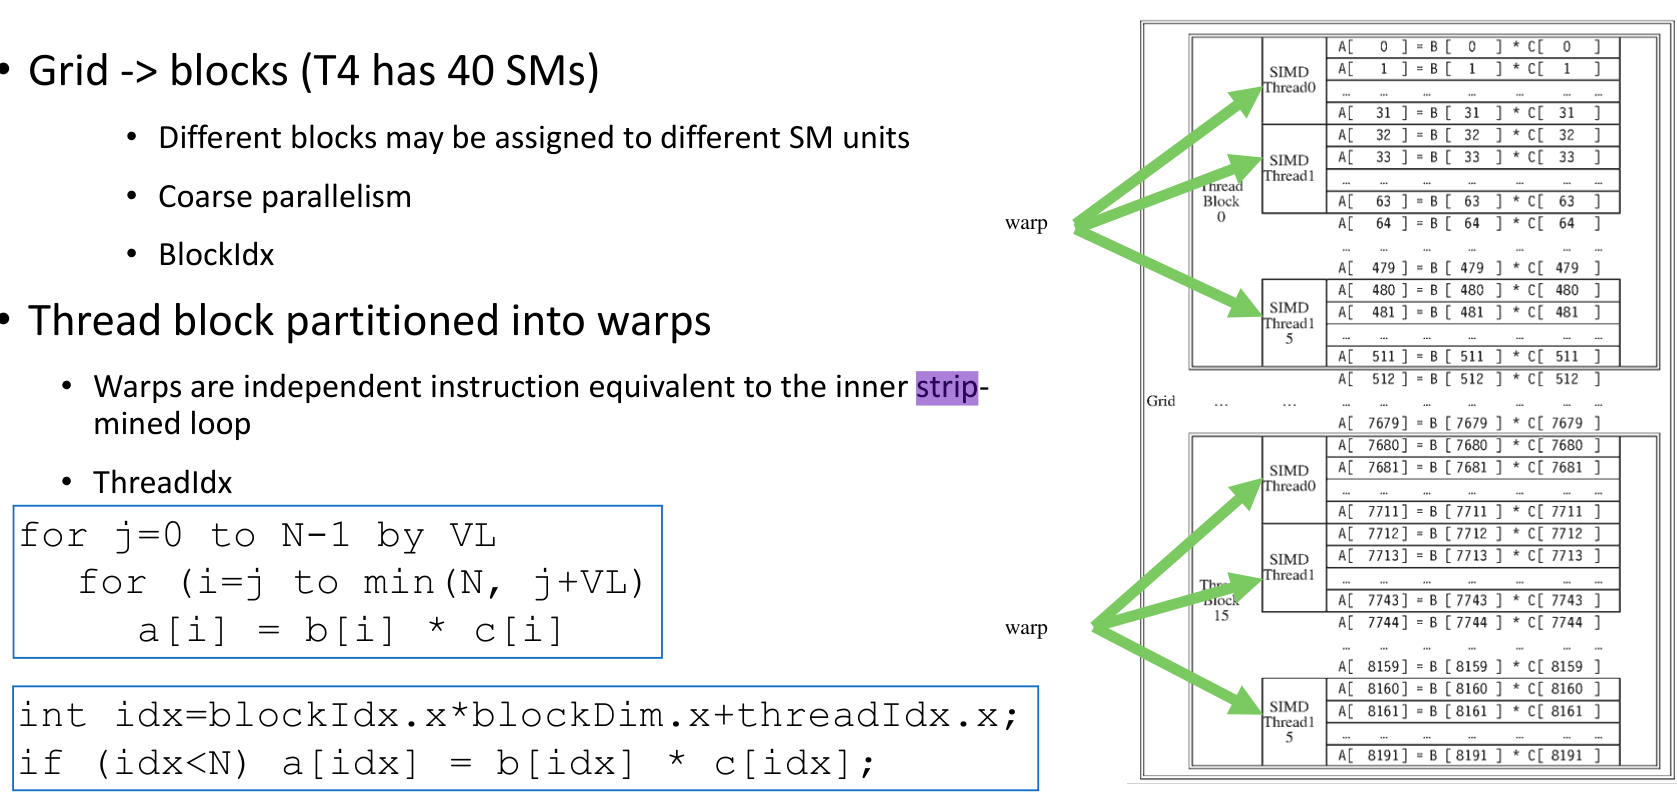
\includegraphics[width=2in]{images/gpu-strip.jpg}
  \end{center}

  – pipelines: big pipe
  \begin{center}
    
\includegraphics[width=2in]{images/pipe.jpg}
  \end{center}

  Pipeline hazards, dependencies: same shit as the multithreading bit but for
  instructions -- go figure -- hazards when instructions resolve before the ones
  before them or some shit dont do that its in the 141 shit i cant be assed. --
  tldr nvcc handles raw instruction hazzards for gpus -- idea came from risc

  CPU pipelines vs GPU pipelines -- bc gpu is for throughput they have the
  biggest pipes

  Emphasis on latency reduction, emphasis on throughput: big pipe

  Scoreboarding in a GPU – detect when dependencies are resolved: tracks warps
  ready to be issued
  \begin{center}
    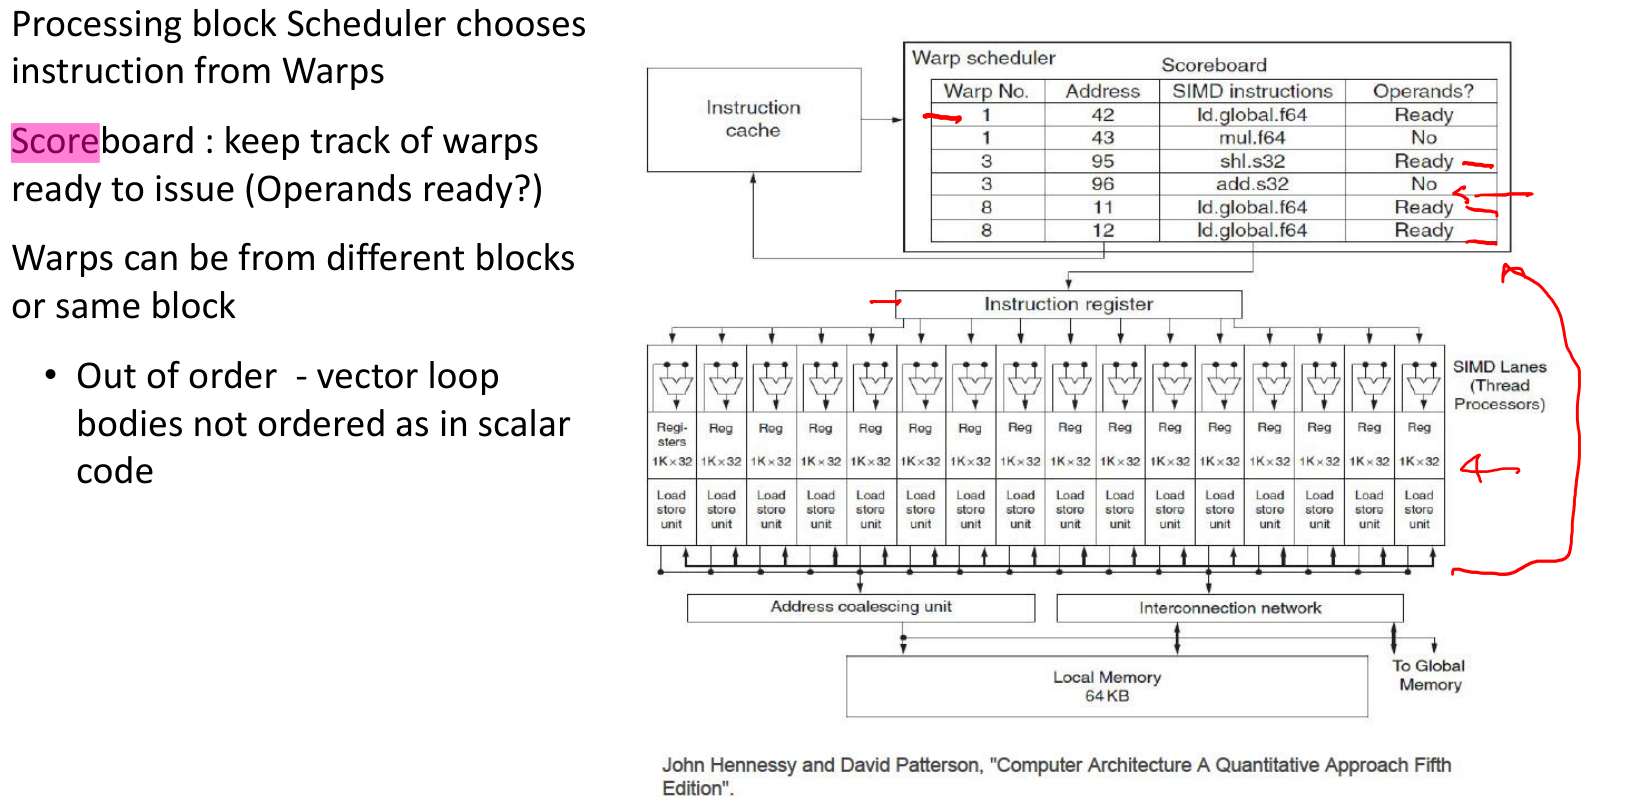
\includegraphics[width=2in]{images/scoreboard.jpg}
  \end{center}



  Reduction operation in a GPU and how to lessen control divergence
  \begin{center}
    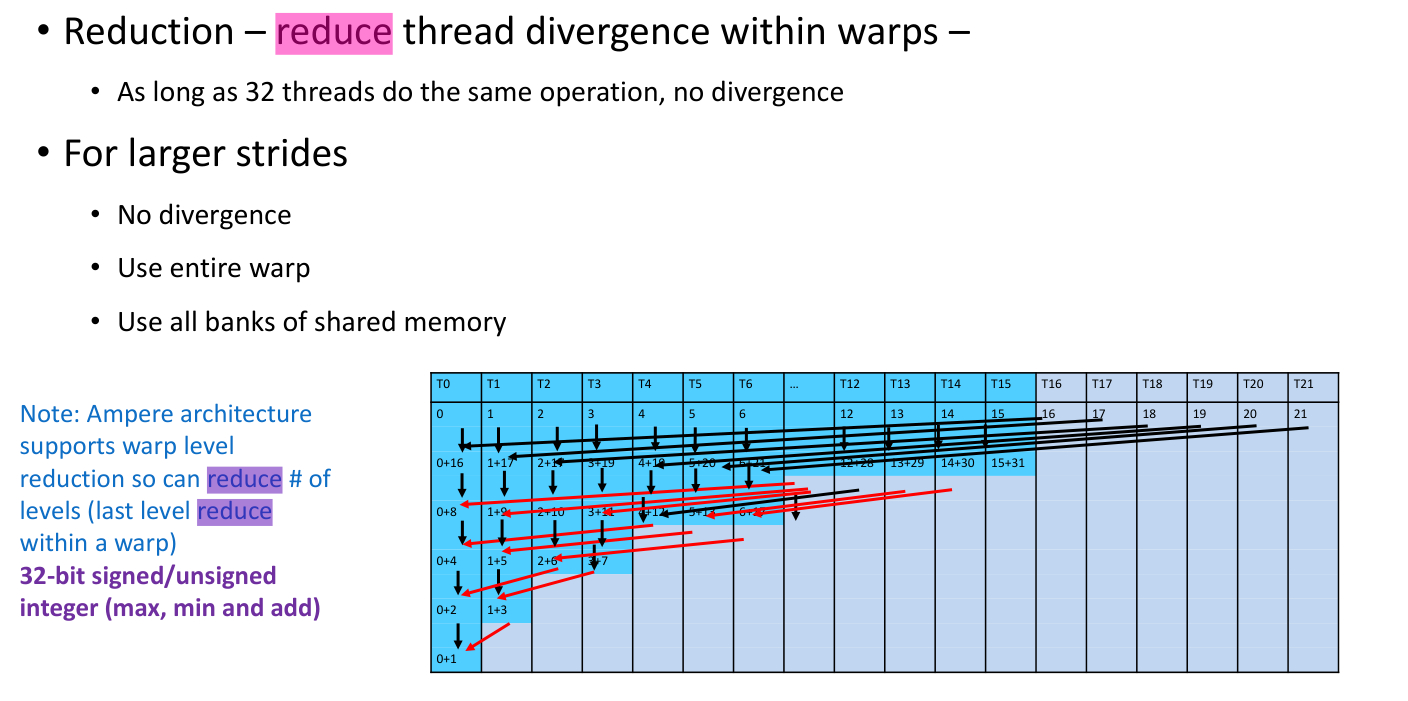
\includegraphics[width=2in]{images/gpu-reduce.jpg}
  \end{center}

  \section{Message Passing}

  Bulk Synchronous: execution exists as 3 phaes - compute, communicate and
  syncronize. works when threads do roughly the same ammount of work. $L$ is
  super step interval. $h$ messages per superstep. $g$ communication cost (1/bw
  + fixed overhead). $T_\text{comm} = gh$ message startup cost is generally
  ignored.

  Stencil Methods: smth smth a think a convolution (rito sue me).

  What kinds of problems are amenable to stencil methods: particle simulation,
  event based simulation -- if it occurs on a grid duh.

  ghost cells: duh -- u did pa3 no?

  Basic MPI concepts : Rank, ordering guarantees/causality, synchronous and 
  asynchronous models. Mpi communicators, mpi tags.: \verb|MPI_Cry|
  \verb|MPI_Bcast|, \verb|Scatter|, \verb|Gather| \verb|Reduce|, etc.  and why you might use them (you don’t 
  need to memorize their detailed behavior, but you should know generally when 
  you might use them).: 
  quirks -- mpi\_barrier only stops all code from continuing after everything on
  the communicator has called it. nonblocking sends and recieves have a status
  struct that can be used to wait on for data validation smth smth mpi\_request.

  Difference in user semantics for blocking and non-blocking send/recv (when you
  can use the buffers, what you have to do to synchronize non-blocking comms):
  deadlocks. mpi\_request structs hf.
  
  under the hood everything exists in some extenral buffer from your code with
  mpi calls. often exists as a kernel buffer somewhere. when sends and recieves
  are resolved then kernel buffer is copied to user data. non blocking comms
  avoid double copy from kernel to user but need for wait or some shit to
  validate send and receives.

  transmit modes or some shit: eager mode -- send message to reciever (reciever
  has to garuntee the kernel buffer landing zone is avaliable there exists some
  limit not sure what it is tho prob mtu size or some shit, rendevous mode --
  query reciever if buffer is avaliable before sending big pipe of data.
   
  One-sided communications: tldr accessing of remote memory as either put
  (writing) or as a get (reading). tldr no explicit sends to reciever -- smt
  hsmth rdma shit. often done with hardware offload. prob a pa3 optimization
  wonder if yuchen will see this. 

  \subsection{MPI Perf modeling}

  $\text{TotalTime} = \gamma \times \#\text{ops}  +  \#\text{msgs} \times (\alpha +
  \beta^{-1}_\infty \times n)$  where $n$ is the msg size, $\alpha$ is message
  latency, $\beta_\infty$ is peak bandwidth and $\gamma$ is time per op.

  \subsection{Communication Parameters}

  \begin{center}
    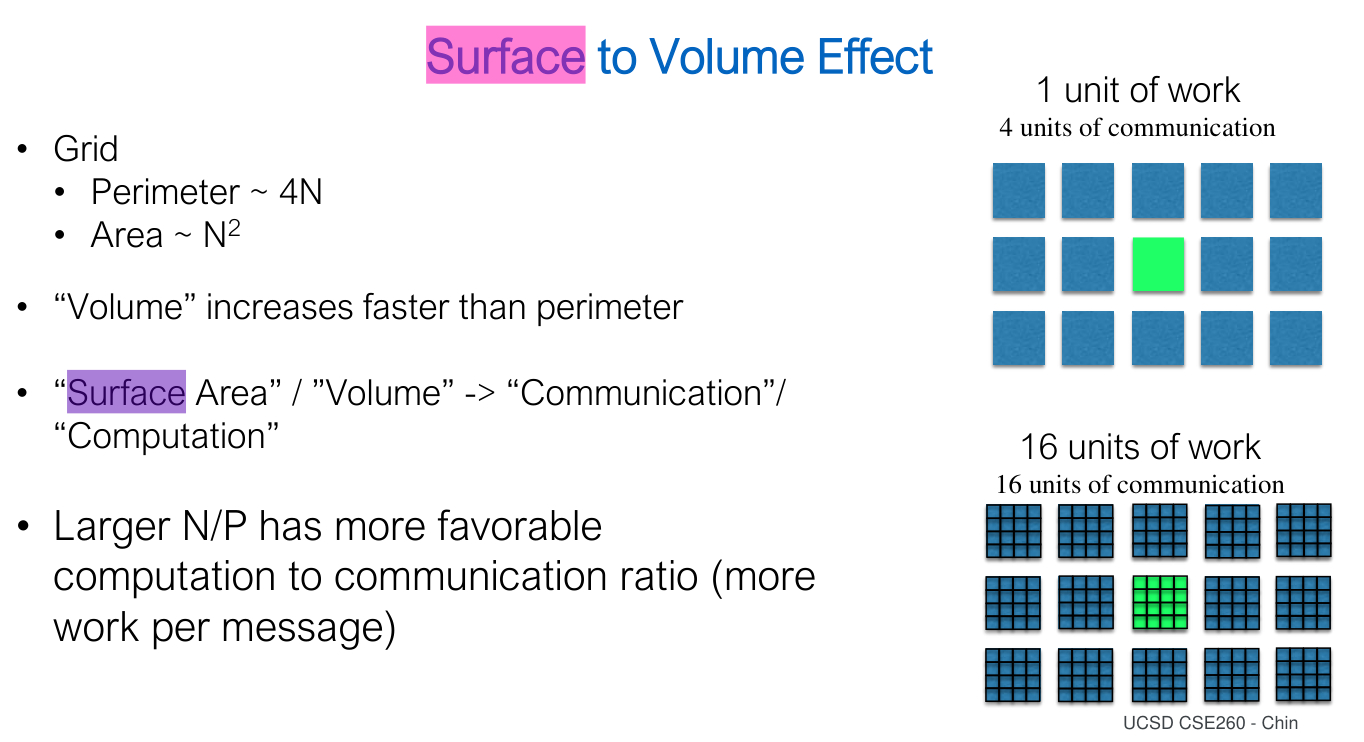
\includegraphics[width=2in]{images/surface-2-vol.jpg}
    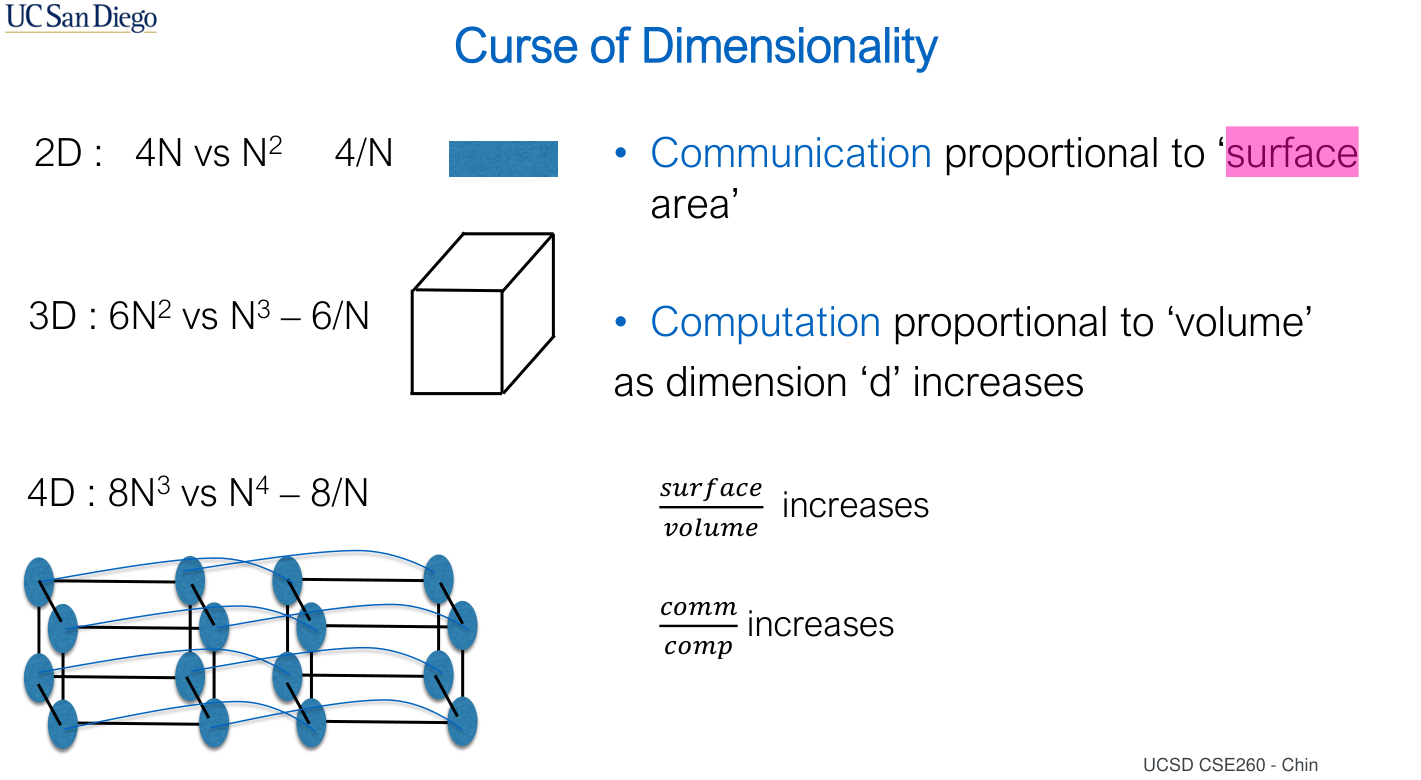
\includegraphics[width=2in]{images/dimentionality.jpg}
  \end{center}
  Effect of higher dimension grid on surface to volume effect.: shit becomes
  more sensitive to processor geometry
  Effect of higher dimensions on cache locality.
  \begin{center}
    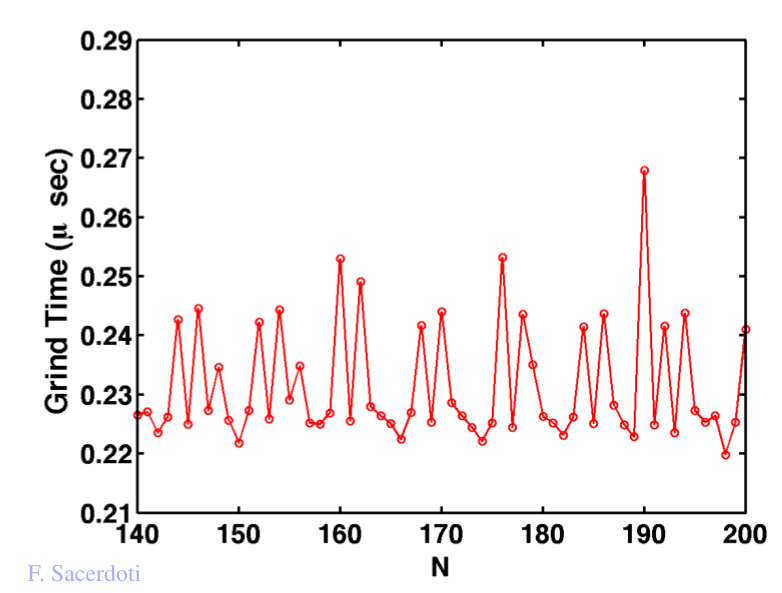
\includegraphics[width=2in]{images/sensitivity.jpg}
  \end{center}

  \section{Asics}


  An Application Specific Integrated Chip is described by its name. Example includes a Switch ASIC for routing, google's TPUs, or any other specially designed Chip

  How systolic array does matrix multiplication:

  Systolic Arrays are similars to registers but while having data flow throw through it apply some operationg to the data flowing through it. 

  MM with a Systolic Array:
  \begin{center}
    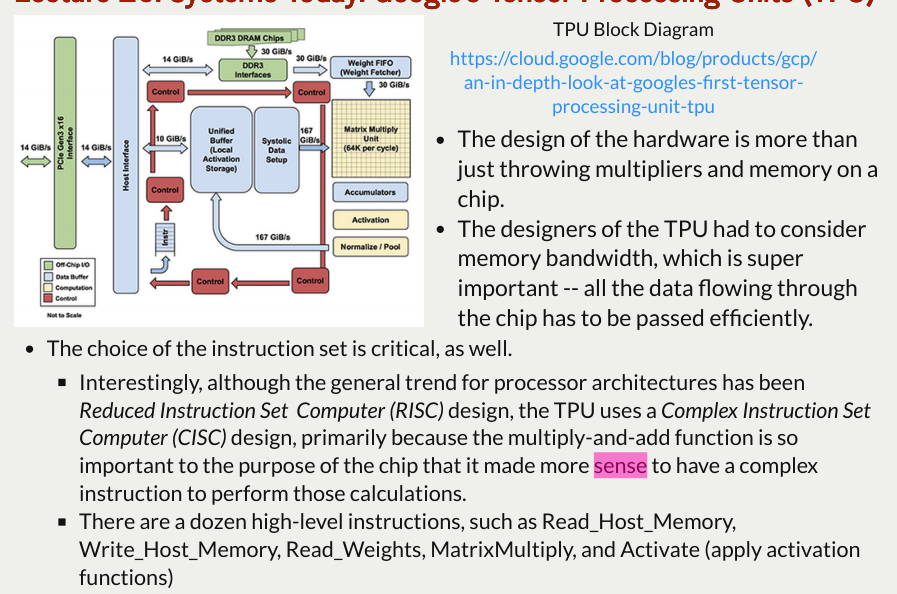
\includegraphics[width=2in]{images/tpu-block.jpg}
    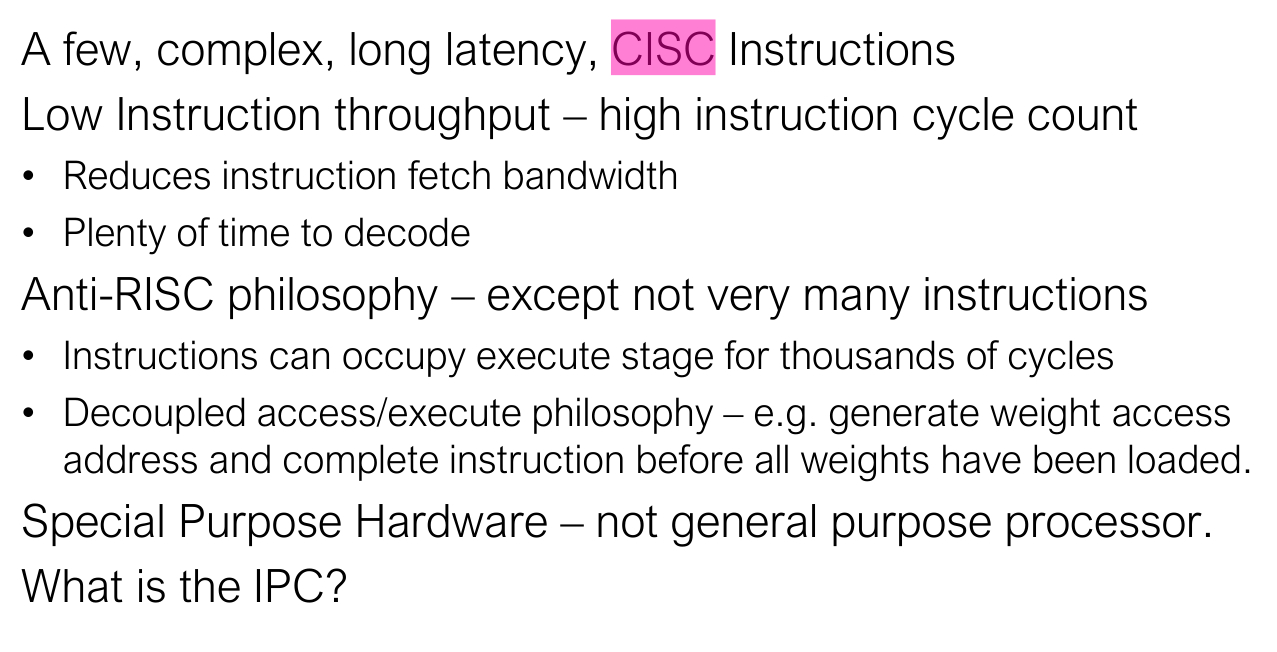
\includegraphics[width=2in]{images/tpu-inst.jpg}
    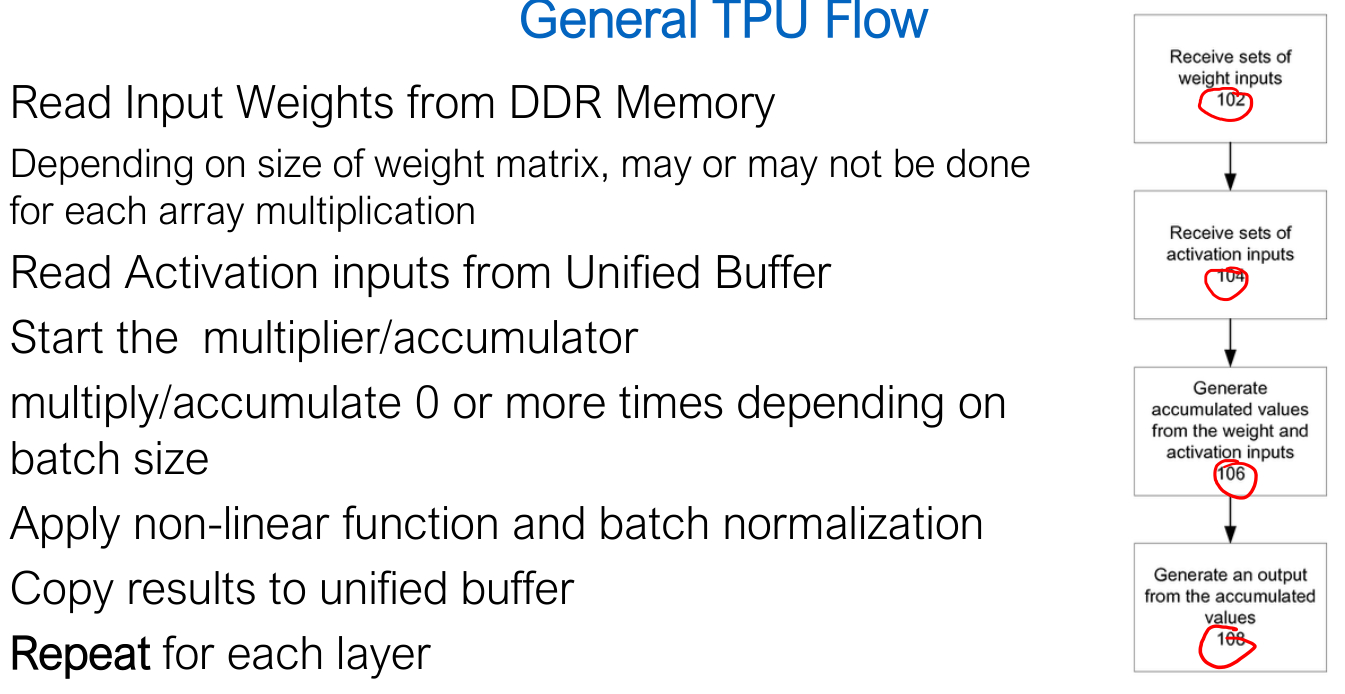
\includegraphics[width=2in]{images/tpu-flow.jpg}
    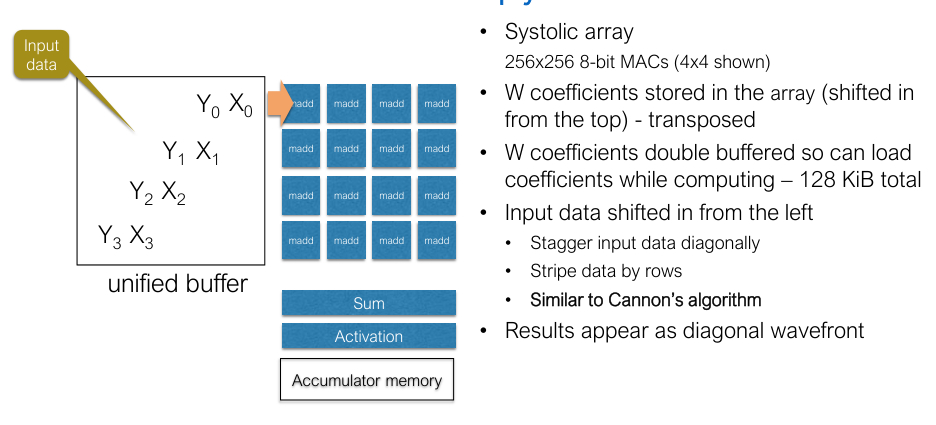
\includegraphics[width=2in]{images/tpu1.jpg}
    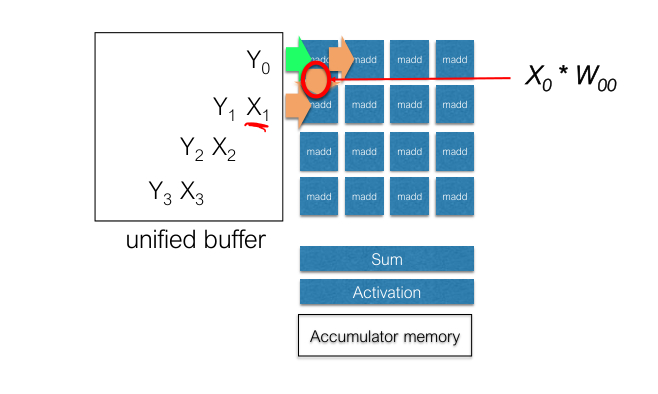
\includegraphics[width=2in]{images/tpu2.jpg}
    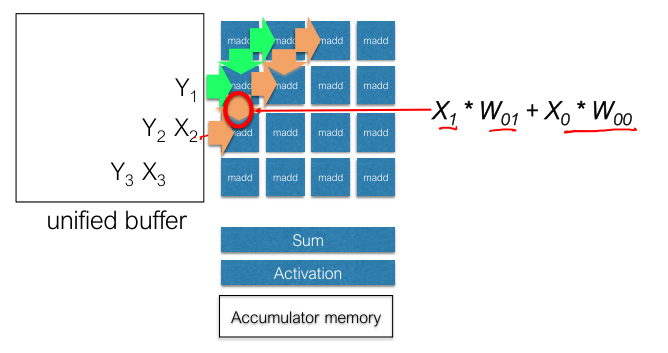
\includegraphics[width=2in]{images/tpu3.jpg}
    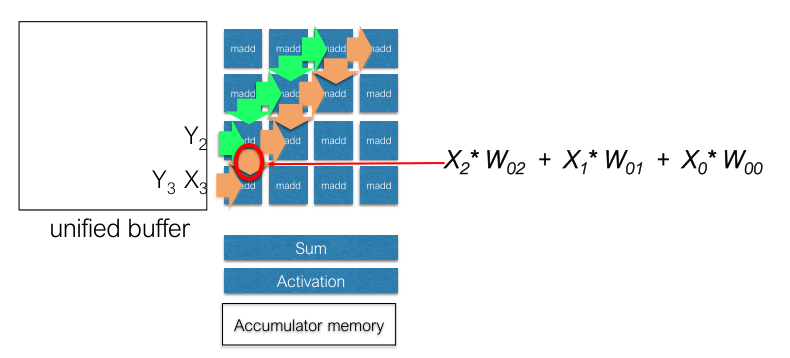
\includegraphics[width=2in]{images/tpu4.jpg}
    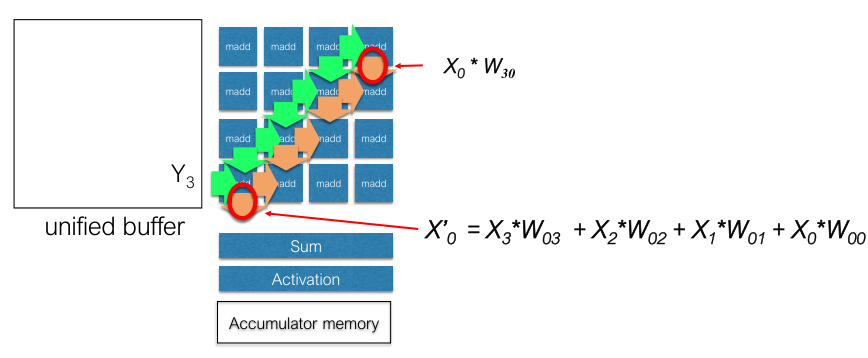
\includegraphics[width=2in]{images/tpu5.jpg}
    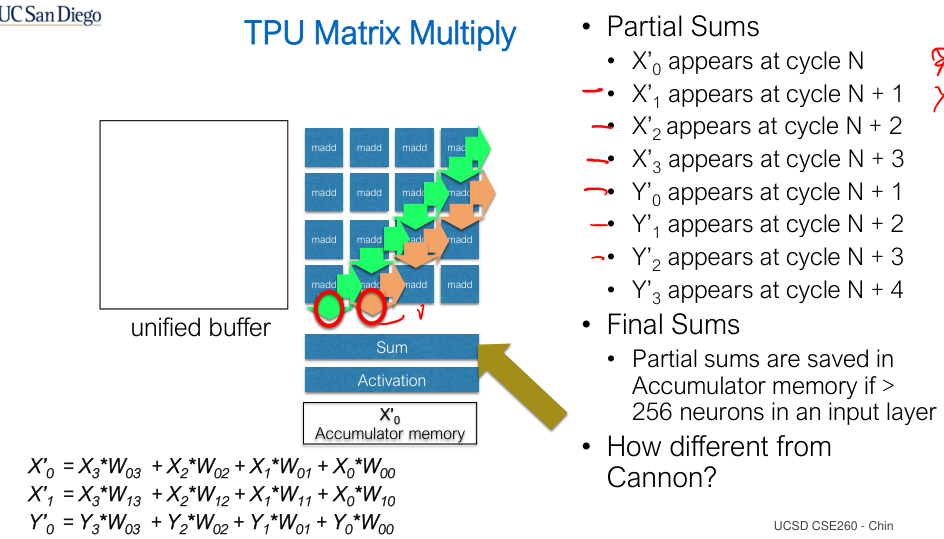
\includegraphics[width=2in]{images/tpu6.jpg}
    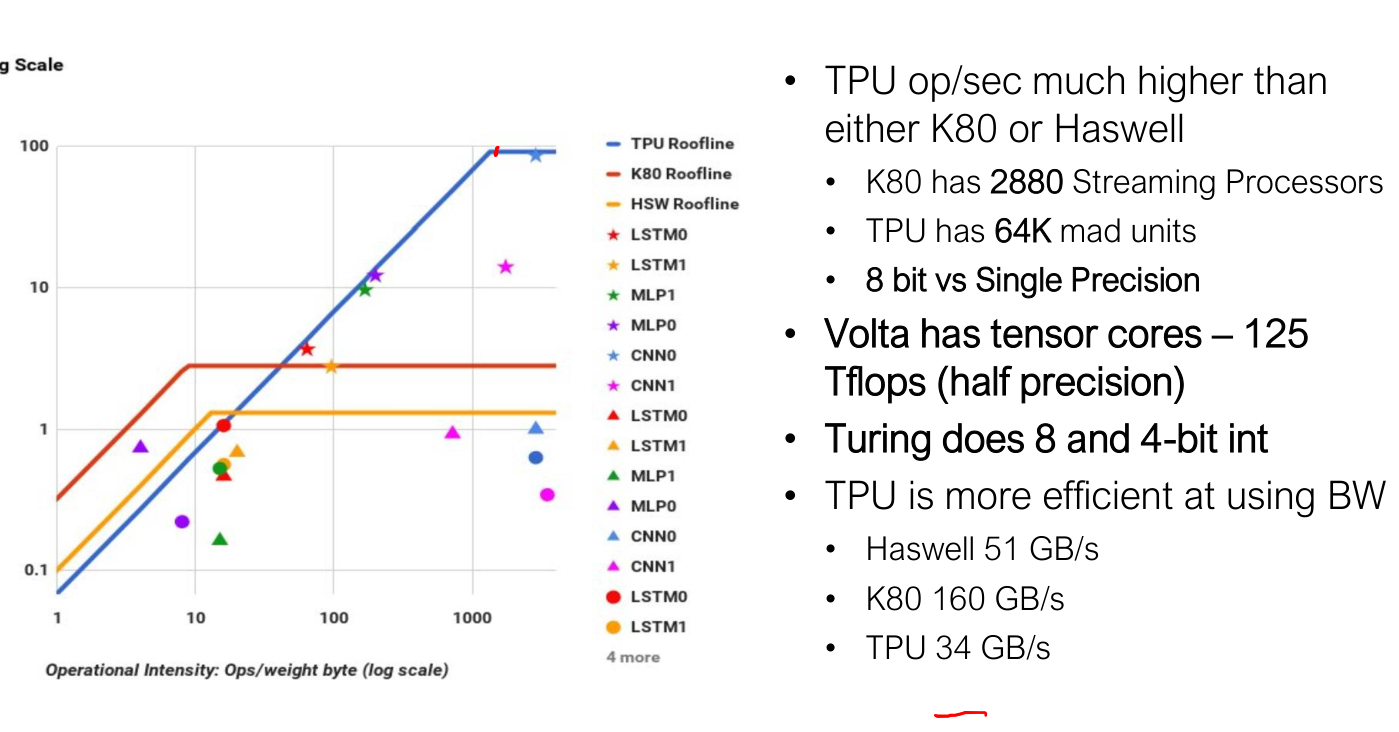
\includegraphics[width=2in]{images/tpu-roofline.jpg}
  \end{center}

  Difference between Canon’s algorithm and TPU’s systolic array: 
  The systolic array elements are being fed into the array
  and ending up a some sum buffer to accumulate over TIME, not immediately, but they are in Canon's.

  Why CISC instructions in the TPU
  Instrucitons need to be complex for the TPU, sometimes spending multiple cycles in decoding and execution. Can generate weights, decouples access/execute philosphy, etc. (Leads to "dogshit ipc")
  
  \section{Higher Level Abstractions}

  Major differences between, pthreads, openMP, Cuda, MPI - fuck you figure it
  out. - Paco \& Khai

  \section{Examples}
  
  none




\end{multicols}

\end{document}

